\chapter{System Design and Verification}

\section{Introduction}

To be able to determine the pose error of a drone in flight, an outdoor pose measurement system is required. Due to their considerable cost, radar and laser measurement systems were not considered, which required another method to be devised. One method that was investigated is a computer vision system (CVS) that can estimate the pose of a drone.

The CV measurement system makes use of a flat calibration pattern and a Perspective n-Points (PnP) problem solver to extract the six-dimensional pose data vector $\bm{x} = {[x\;y\;z\;\theta\;\phi\;\psi]}^T$, where ${[x\;y\;z]}^T$ are the translation dimensions and ${[\theta\;\phi\;\psi]}^T$ are the roll, pitch and yaw dimensions respectively. 

This section discusses the details of CVS that was investigated and implemented. It starts by discussing the system layout and design

\section{Computer Vision System Layout}

\subsection{Hardware}

The hardware requirements for the CVS are minimal. To perform six-dimensional pose estimation of a calibration pattern, either one or two cameras are required, along with a flat board containing the calibration pattern and a laptop running the pose estimation software. 

The accuracy between the single and stereo camera in most respects is rather negligible, except in the depth dimension, where the stereo vastly outperforms the single camera. This is to be expected and is very akin to a person's depth perception abilities being compromised with one eye closed. For this implementation, the single camera variant was selected. This makes the system simpler to set up and use. However, care must be taken with the depth estimation when using a single camera. In the future, the project can be expanded to a stereo camera system.

For the pose estimation software to work best, it requires a clear view of the calibration pattern. Therefore, a big calibration pattern is desirable. Furthermore, the pattern should of a high quality and printed on white paper with a wide white border to enhance the contrast between the pattern and the background, making it easier for the software to detect the pattern. 

\subsection{Software}
\label{sec:cv-sys-software}

The software used to perform the pose estimation comes packaged with the OpenCV computer vision library. 

The camera of the CV system is calibrated by a calibration function and pattern. The goal of the calibration process is to determine the intrinsic parameters of the camera matrix. The camera matrix takes up the form given in Equation~\ref{eq:cam-matrix}

\begin{equation}
  \label{eq:cam-matrix}
  C = 
  \begin{bmatrix}
    f_x & 0   & u_0 \\
    0   & f_y & v_0 \\
    0   & 0   & 1   \\
  \end{bmatrix}
  \begin{bmatrix}
    R | T
  \end{bmatrix}
\end{equation}

where $f_x$ and $f_y$ describe the focal lengths of the camera, and $u_0$ and $v_0$ are the principal points. $R$ is a $3\times3$ matrix describing the rotation of the camera, and $T$ is a three-dimensional vector describing the translation of the camera. 

To extract data from the image of a calibration board, a feature detection function from OpenCV was used. It scans the image and returns a set of two-dimensional data points of the features, i.e.\ coordinates of some predefined shape or form, of the calibration pattern. Then, a Random Sample Consensus (RANSAC) algorithm is used to discard any erroneous data points.

The transformation from two-dimensional image coordinates, $\bm{x}_c$, to to three-dimensional world coordinates, $\bm{x}_w$, is given by Equation~\ref{eq:2d-to-3d}.

\begin{equation}
   \label{eq:2d-to-3d}
   \begin{bmatrix}
     x_c & y_c & 1 \\
   \end{bmatrix}^T
   = C
   \begin{bmatrix}
     x_w & y_w & z_w & 1 \\
   \end{bmatrix}^T
 \end{equation}

With the camera matrix $C$ known, and a set of two-dimensional data points, a Principle n-Point (PnP) problem solving function can be used to extract the $R$ and $T$ matrices, describing the pose of the camera relative to the calibration board, from the data. The standard PnP solver, as described by~\cite{Schweighofer2006}, is used. The Efficient-PnP method, described by~\cite{Lepetit2008}, is more efficient, but requires more data points, which a typical calibration board may not have many of.

\section{Measurement Test Design}

Before the CVS was used to record the pose data of a drone, the accuracy of the system's measurements was first determined. Since the PnP solving algorithm is, at its core, an optimisation problem and produces estimates of the pose, determining the accuracy of the CVS is an important step in the system design phase. 

To determine the measurement error, a measurement test was performed in an indoor environment where an external measurement device recorded pose data. The error was then be determined by comparing the CVS's data with that of the external measurement system's measurement data. Both systems were set to record the pose of a flat chessboard calibration pattern that was moved and orientated by hand.

This section describes the test layout, including the external measurement device and its details, as well as the CVS details. Then, the measurement procedure is presented, followed by the steps taken to process the data during the post-processing phase. Finally, the results of the test are given and discussed. 

\subsection{Test Layout}
\label{sec:vicon-test-setup}

\subsubsection{External Measurement Device Layout}

The external measurement system used to record the data that was used as ground-truth pose data, is a Vicon indoor motion capture system. It is a widely-used commercial system with applications in the film, medical and sporting industries and can reach sub-millimetre accuracy in its measurements. It works by tracking a set of infrared markers stuck to a surface with at least two infrared cameras and sophisticated proprietary motion tracking software. Given its accuracy, the measurement results from this system was taken as ground-truth.

The Vicon system used for the test is located in the 3D Human Motion Laboratory on Stellenbosch University's Tygerberg medical campus. It consists of eight infrared cameras arranged around a square on the floor in a configuration that maximises the number of infrared markers visible to each camera at any given point in time. Figure~\ref{fig:vicon-layout} shows a diagram of the Vicon system layout. 
 
\begin{figure}
  \centering
  \def\svgwidth{0.6\textwidth}
  \input{figures/chapter3/vicon_layout.pdf_tex}
  \caption[Layout of the Vicon motion capture system.]{Layout of the Vicon motion capture system. Note that this is not drawn to scale.}
\label{fig:vicon-layout}
\end{figure}

Before the test commenced, the Vicon system was calibrated and the infrared markers were placed on both the calibration board and camera frame used by the CVS\@. Since the Vicon and CVS camera each have their own coordinate systems, having the position and orientation of the CVS camera available will allow the Vicon's measurements to be related back to the CVS's camera coordinate system during the post-processing phase. The markers were placed in such a way that they will produce axes that more or less coincides with the Vicon's axis system, slightly reducing the work load during the post-processing phase. Figure~\ref{fig:cam-vicon-axes} shows the axis system's for both the CVS and Vicon systems.

\begin{figure}
  \centering
  \def\svgwidth{0.6\textwidth}
  \input{figures/chapter3/cam_vicon_axis.pdf_tex}
  \caption{The axis orientations of the Vicon and CV systems.}
\label{fig:cam-vicon-axes}
\end{figure}

Only three markers are required for the Vicon system to produce a six-dimensional pose vector, but a fourth asymmetrical auxiliary marker was placed to provide fail-safe orientation data during the post-processing phase. Figures~\ref{fig:cam-marker-placement} and~\ref{fig:board-marker-placement} show the marker placements for the camera and calibration board. These markers were carefully placed by hand, but there will be some placement error nonetheless. This error offset is taken into account during the data processing phase. 

\begin{figure}
   \centering 
   \includegraphics[clip, trim = 0 400 0 400, width=0.8\textwidth]{figures/chapter3/cam_1.pdf}
   \caption{Infrared marker placement on the camera.}
\label{fig:cam-marker-placement}
\end{figure}

%\begin{figure}
   %\centering 
   %\includegraphics[clip, trim = 600 0 400 0, width=0.8\textwidth]{figures/chapter3/bord_2.pdf}
   %\caption{Infrared marker placement on the chessboard.}
%\label{fig:board-marker-placement}
%\end{figure}

One aspect of the Vicon system to note is that the infrared markers have some high-frequency noise associated with them, which is apparent when inspecting the raw data. This noise is inherent to the marker and can be safely filtered out with a zero-lag, second order Butterworth filter. However, the raw, unfiltered data is used throughout this project. 

\subsubsection{Computer Vision System Setup}

The CVS consists out of a single Microsoft LifeCamHD webcam, capable of recording 720p High-Definition (HD) video data at 30 frames per second (FPS), an A1, $5\times6$ square chessboard pattern, generated by OpenCV's pattern generator, and a laptop running the software required to capture video. The webcam's focal length, image resolution, FPS rate and exposure can be controlled from a laptop. 

Before the test, the camera was calibrated to determine its camera matrix and focal lengths in the $x$ and $y$ directions. Calibration was done with the same board and camera that was used during the test, against a white, well-lit background. The board was moved to different positions and orientations within view of the camera, and roughly 15 still images in standard resolution ($640\times480$ pixels) were taken. The camera was then calibrated with this set of images and OpenCV's camera calibration module to produce a camera matrix that gives a reprojection error of between 0.18 and 0.21 pixels. 

In the test, the camera was placed in a stable aluminium frame and was left untouched throughout the test. The laptop was set to only capture video at $640\times480$ pixels, while zoom and autofocus was disabled to keep the camera's focal lengths to the constant focal length that was determined during calibration, which is approximately 700 pixel units. The data extraction and pose estimation took place off-line. 

\subsection{Test Procedure}

Figure~\ref{fig:pic-sys-layout} shows a picture of the complete setup. As described in Section~\ref{sec:vicon-test-setup}, the camera is placed on a chair and the board is held facing the camera. Both of these are covered with four infrared markers with the eight infrared cameras surrounding both the board and camera.  

%\begin{figure}
  %\centering
  %\includegraphics[clip, trim = 600 300 0 0, width=0.8\textwidth]{figures/chapter3/sys_1.pdf}
  %\caption{Picture of the test layout.}
%\label{fig:pic-sys-layout}
%\end{figure}

Data capture started when the Vicon system started recording. At the same time, the chessboard was tilted forward. This allowed for the data to be synchronised to a common timeframe during the data processing phase. During the data capturing phase, the board was moved by hand to different positions and orientations with respect to the camera's axis system, to generate data vectors. To produce a diverse cloud of data vectors, the board was moved around the full field of view and depth of the camera, while varying the rotational orientation at the same time. Each video is approximately 90 seconds long, which equates to close to 2700 pose vector samples per test, though it was decided that only 2400 of these points will be used for consistency reasons. 

The test produces two sets of data: one ground-truth pose measurement data set from the Vicon system, and one data set from the CVS\@. These data sets allows the determination of the CVS measurement error. These sets were also used to provide training and validation data sets for a error prediction mode, which is discussed in Section MEMEMEMEME.\@

\subsection{Data Processing}

During the test, the CVS only captured video data, leaving the data extraction and pose estimation to be done off-line during the data processing phase. The Vicon system data requires very little processing, since most of the data is generated in real-time and is optimised by the Vicon software. However, some work was done to fix incorrect measurements that were introduced when not enough Vicon cameras have a good view of the infrared markers. These points were corrected by means of interpolation. Furthermore, since the CVS data is the focus of these tests, the Vicon system's axis system was rotated and reorientated to coincide with the axis system of the CVS.\@

Processing the CVS data involves several steps, which include simultaneously optimising the camera's focal length and the infrared marker offsets and then determining the accuracy of the CVS pose estimation system. Each of these aspects are discussed next.

\subsubsection{Rotating the Camera and Chessboard Data}
\label{sec:rotate-axes}

During the test, four markers were placed on the CVS camera frame to provide data on its placement. These markers were placed along the camera's $x$ and $y$ axes and is identical to the chessboard's axis system. 

With the CVS's camera placement and orientation in the Vicon coordinate system known, it is possible to move the Vicon axis system to the centre of the CVS's camera axis system and to find the angle between the Vicons's axis system and the CVS's camera. This was done by finding the $\arctan$ relationship between the relevant axes and was double checked by using the cosine angle of the dot product. As an additional sanity check that the measurements are correct, the angles have to be relatively constant, since the camera does not move during the experiment. This was indeed the case, except for some high-frequency sensor noise introduced from the Vicon system, which may ignored given its small magnitude. 

With the angular deviation between the Vicon and CVS's camera axis system's known, an Euler rotation matrix of type 1--2--3 can be set up. This matrix can then be used to rotate the Vicon's measurement data of the calibration board to coincide with the CVS's camera axis system, making it possible to directly relate the calibration board measurements of the two systems. 

Similarly, it is advantageous to centre the CVS's camera axis system around the Vicon system's origin. This was done by subtracting the CVS's camera Vicon position data from the calibration board and CVS's camera position data given by the Vicon system. This will centre both the Vicon and CVS camera data sets around the Vicon's origin, simplifying the optimisation procedure discussed next. 

\subsubsection{Camera Parameter Optimisation}
\label{sec:focal-optimisation}

Before the test took place, the CVS camera was calibrated using OpenCV's camera calibration toolbox. This procedure provides a fairly good estimate of the intrinsic parameters of the camera, e.g.\ the focal lengths. However, given the lack of reference three-dimensional data, it is only an estimate. Using the ground-truth Vicon pose data will allow the focal length to be determined more accurately. At the same time, the distance offset between the true infrared marker centre and the ideal infrared marker centre also needs to be taken into account. This offset will also account for any constant measurement bias introduced by the CVS\@. This presents a circular optimisation problem: the focal length will affect the perceived offset, while the offset will affect the CVS pose estimates, which in turn affects the ideal focal length. To find the offset and optimum focal length, a dual optimisation strategy was implemented.  

First, the optimisation algorithm is formulated. Suppose $\bm{P}^*$ denotes the six-dimensional pose vector as given by the Vicon system, while $\bar{\bm{P}}$ is the constant offset vector and the subscripts $c$ and $b$ represent the camera and board respectively. $\bm{\epsilon}$ is the error between the Vicon and CV systems' measurements that needs to be determined and $\bm{F}(f)$ is the pose vector measured by the CV camera, as a function of its focal lengths $f_x$ and $f_y$. The Vicon pose and offset vectors are then given by the following equations

\[
  \bm{P}^* = \bm{P}^*_b - \bm{P}^*_c
\]

\[
  \bar{\bm{P}} = \bar{\bm{P}}_b - \bar{\bm{P}}_c
\]

The equation for the pose estimate given by the CVS is 

\[
  \bm{F}(f) = \bm{P}^* - \bar{\bm{P}} + \bm{\epsilon}
\]

which can then be simplified to 

\begin{equation}
  \label{eq:pose}
  \bm{F}(f_x, f_y) = (\bm{P}^*_b - \bar{\bm{P}}_b) - (\bm{P}^*_c - \bar{\bm{P}}_c) + \bm{\epsilon}
\end{equation}

Equation~\ref{eq:pose} forms the basis of the optimisation algorithm.

Next, the constant offset is determined for a constant focal length. The initial focal length is taken to be the focal length given by the calibration procedure (approximately 700 pixel units). The offset is then determined by 

\[
  \sum\limits_i \bm{F}_i(f) - \sum\limits_i(\bm{P}^*_{b,i} - \bm{P}^*_{c, i}) = i\bar{\bm{P}} + \sum\limits_i\bm{\epsilon}_i
\]

At this point, it is assumed that the error vector $\bm{\epsilon}$ is normally distributed around $0$, thereby eliminating it's sum and leading to Equation~\ref{eq:offset}. This assumption will be verified in Section~\ref{sec:err-norm-test}. 

\begin{equation}
  \label{eq:offset}
  i\bar{\bm{P}} = \sum\limits_i \bm{F}_i(f) - \sum\limits_i(\bm{P}^*_{b,i} - \bm{P}^*_{c, i})
\end{equation}

Using the constant $\bar{\bm{P}}$ produced by Equation~\ref{eq:offset}, it is now possible to minimise the error $\bm{\epsilon}$ from Equation~\ref{eq:pose} by varying the focal lengths, $f_x$ and $f_y$. The minimum focal lengths were found by first setting up a $3\times n$ error matrix, consisting of the three translation dimensions, ${[x\;y\;z]}^T$, where $n$ is the number of samples in the data set. The optimisation is based on these three dimensions, since it was found that including the rotation dimensions added too much instability to the procedure. The error matrix is produced by the equation

\begin{equation}
  \label{eq:error-base}
  \bm{\epsilon} = \bm{F}(f) - \bm{P}^* - \bar{\bm{P}}
\end{equation}

Using the $3\times n$ error matrix found in Equation~\ref{eq:error-base}, an error vector is generated by summing the matrix along its columns. The optimum focal lengths are then found by taking the focal length combination that produces the smallest 2-norm of the error vector $\bm{\epsilon}$. The equation looks as follows:

\begin{equation}
  \label{eq:err-min}
  \min_{f_x, f_y}\left \Vert \sum_i  \bm{\epsilon}_i \right \Vert
\end{equation}

With the optimal focal length now determined, the process starts again from Equation~\ref{eq:pose}, finding a new offset for the new focal length. This procedure is iterated a set number of times, minimising the total error norm. After the optimum focal length combination was found, that combination was used in the camera matrix that extracted the pose data from the video data.

In summation, the algorithm is as follows:

\begin{enumerate}
  \item Initialise focal lengths
  \item Repeat $k$ times:
  \begin{enumerate}
    \item Find $\bar{\bm{P}}$ for a constant $f_x$ and $f_y$ (Equation~\ref{eq:offset})
    \item Determine the error vector $\bm{\epsilon}$ with new $\bar{\bm{P}}$ (Equation~\ref{eq:error-base})
    \item Update focal lengths $f_x$ and $f_y$ with focal length that minimises $\left \Vert \bm{\epsilon} \right \Vert$ (Equation~\ref{eq:err-min})
  \end{enumerate}
  \item Use new focal lengths to estimate the chessboard's pose
\end{enumerate}

\section{Results}

During the optimisation procedure, it was assumed that $\bm{\epsilon}$ was normally distributed around 0. In this section, it is proven that this is indeed the case. Convergence of the optimisation procedure is also proven, and the results of the CVS's pose estimates are presented and discussed.

\subsection{Proof of Convergence}

To test for convergence, the total error for each dimension after an entire iteration of the optimisation was determined and plotted. Figure~\ref{fig:err-convergence} shows the errors of the $\bm{\epsilon}$ vector over 50 iterations.

\begin{figure*}
  \centering
  \begin{subfigure}{0.45\textwidth}
    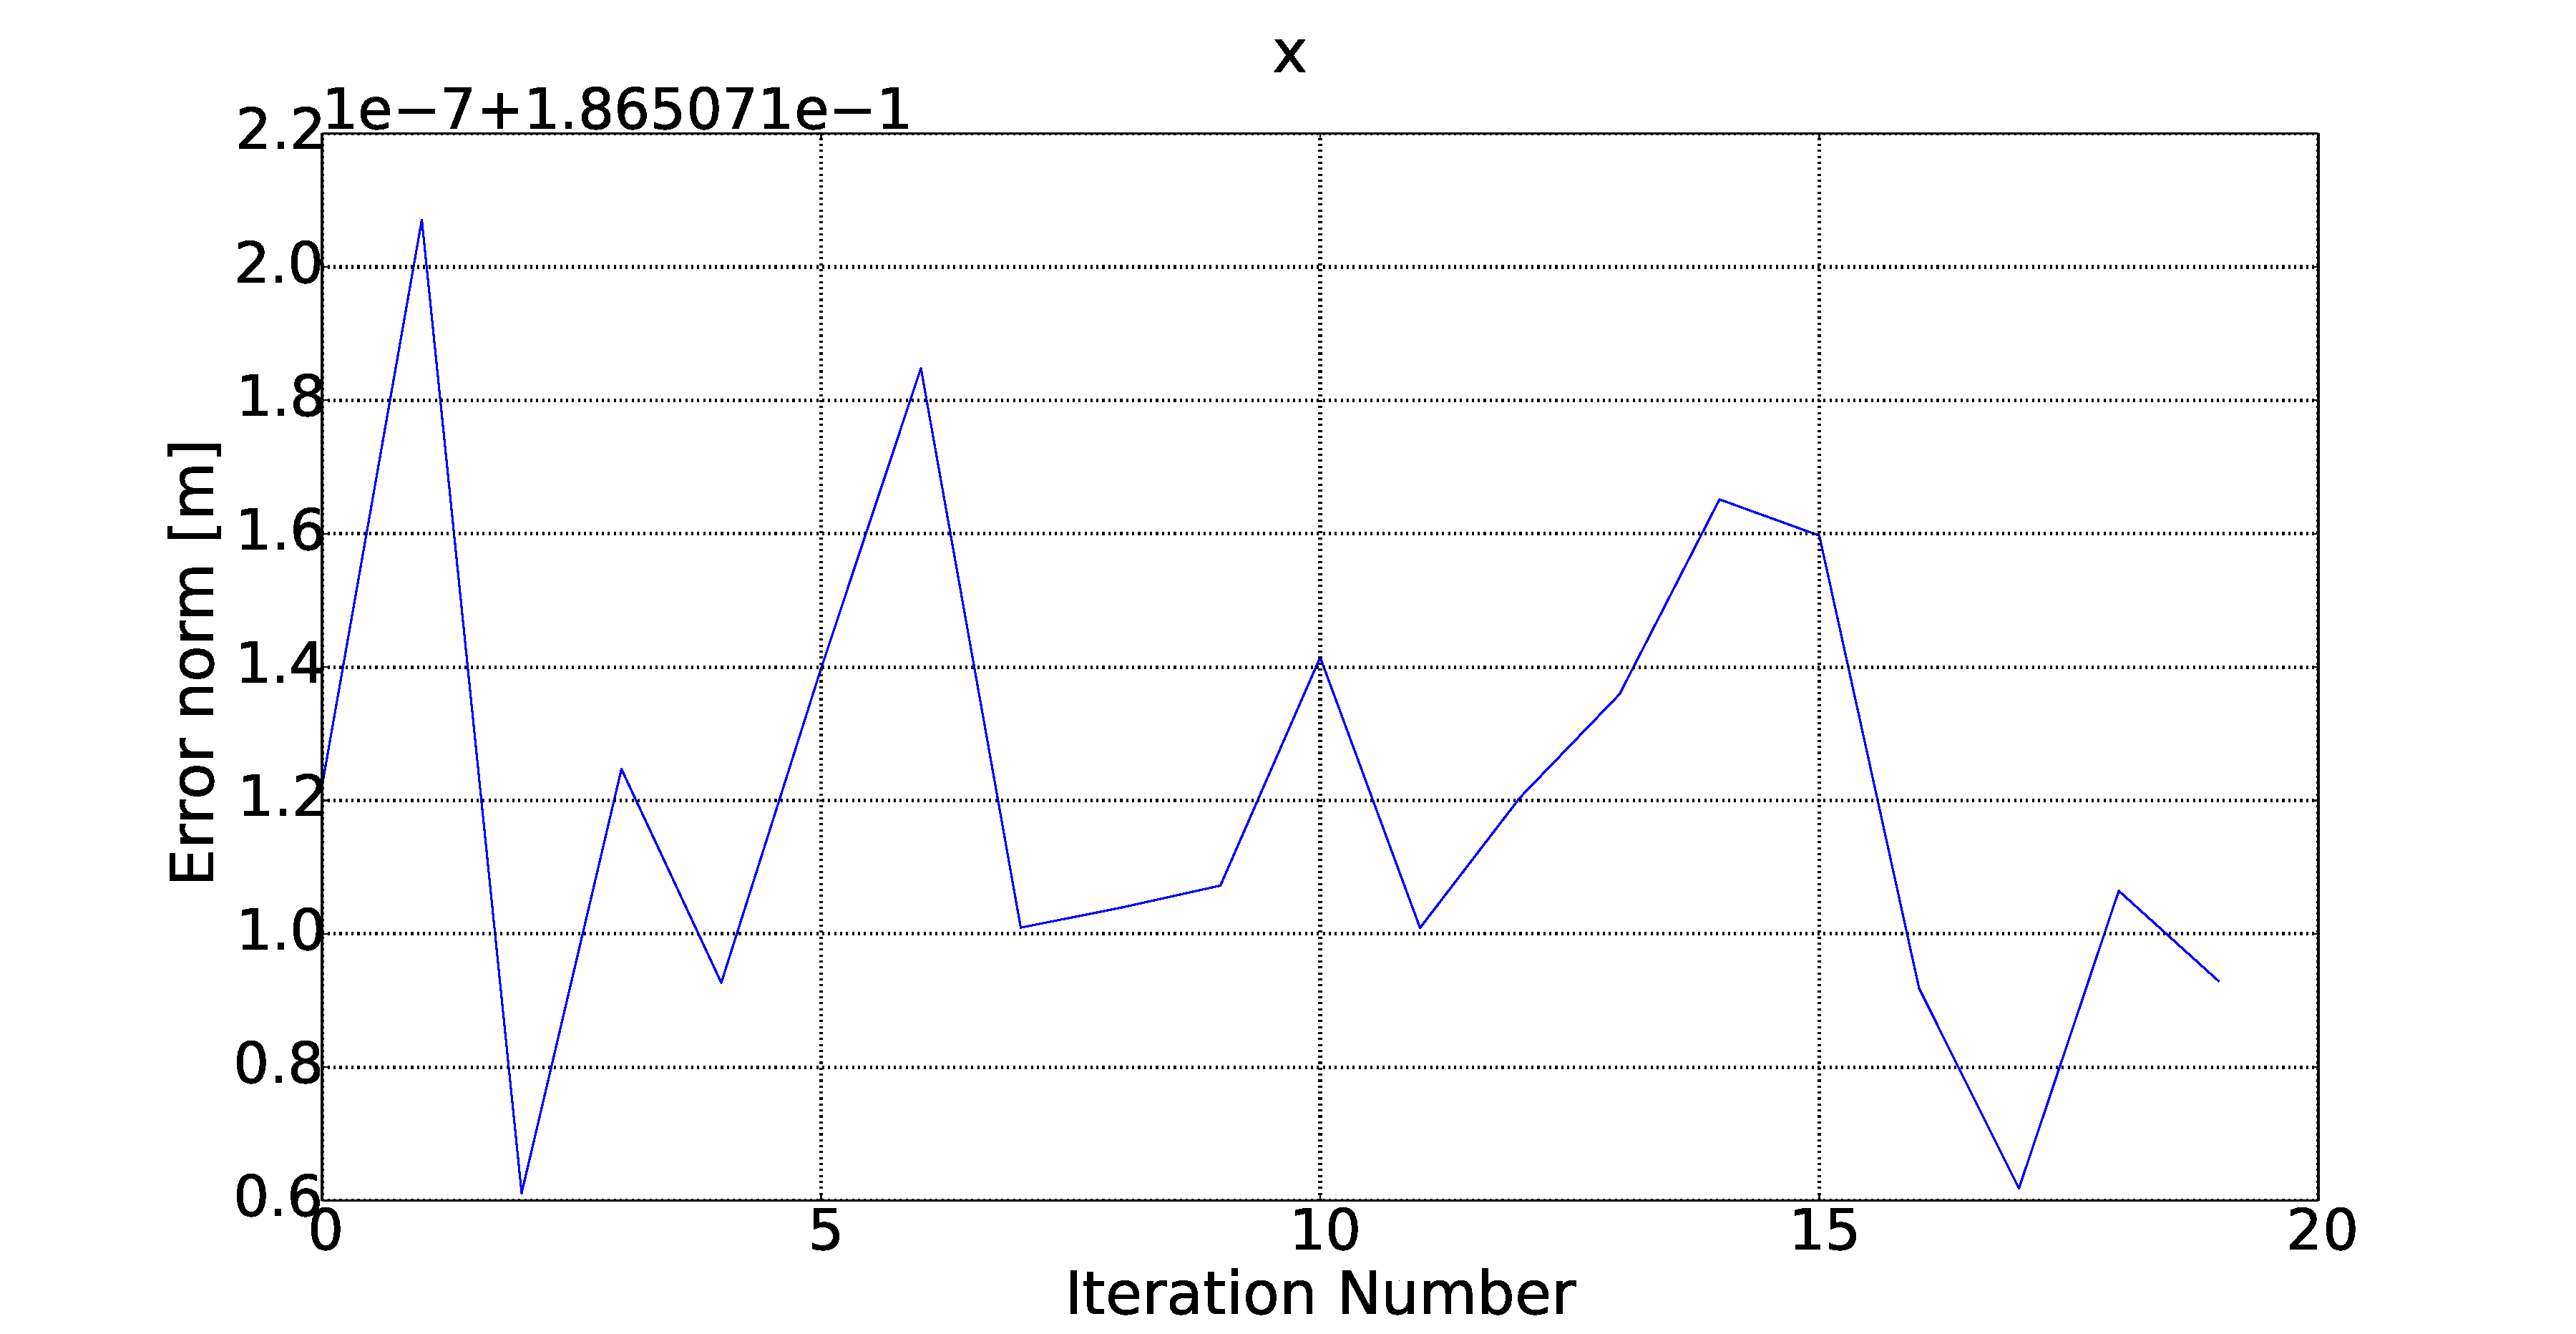
\includegraphics[width=\textwidth]{figures/chapter3/err_x.pdf}
    \caption{Error convergence in the $x$ dimension [m].}
\label{fig:err-convergence-x}
  \end{subfigure}
~
  \begin{subfigure}{0.45\textwidth}
    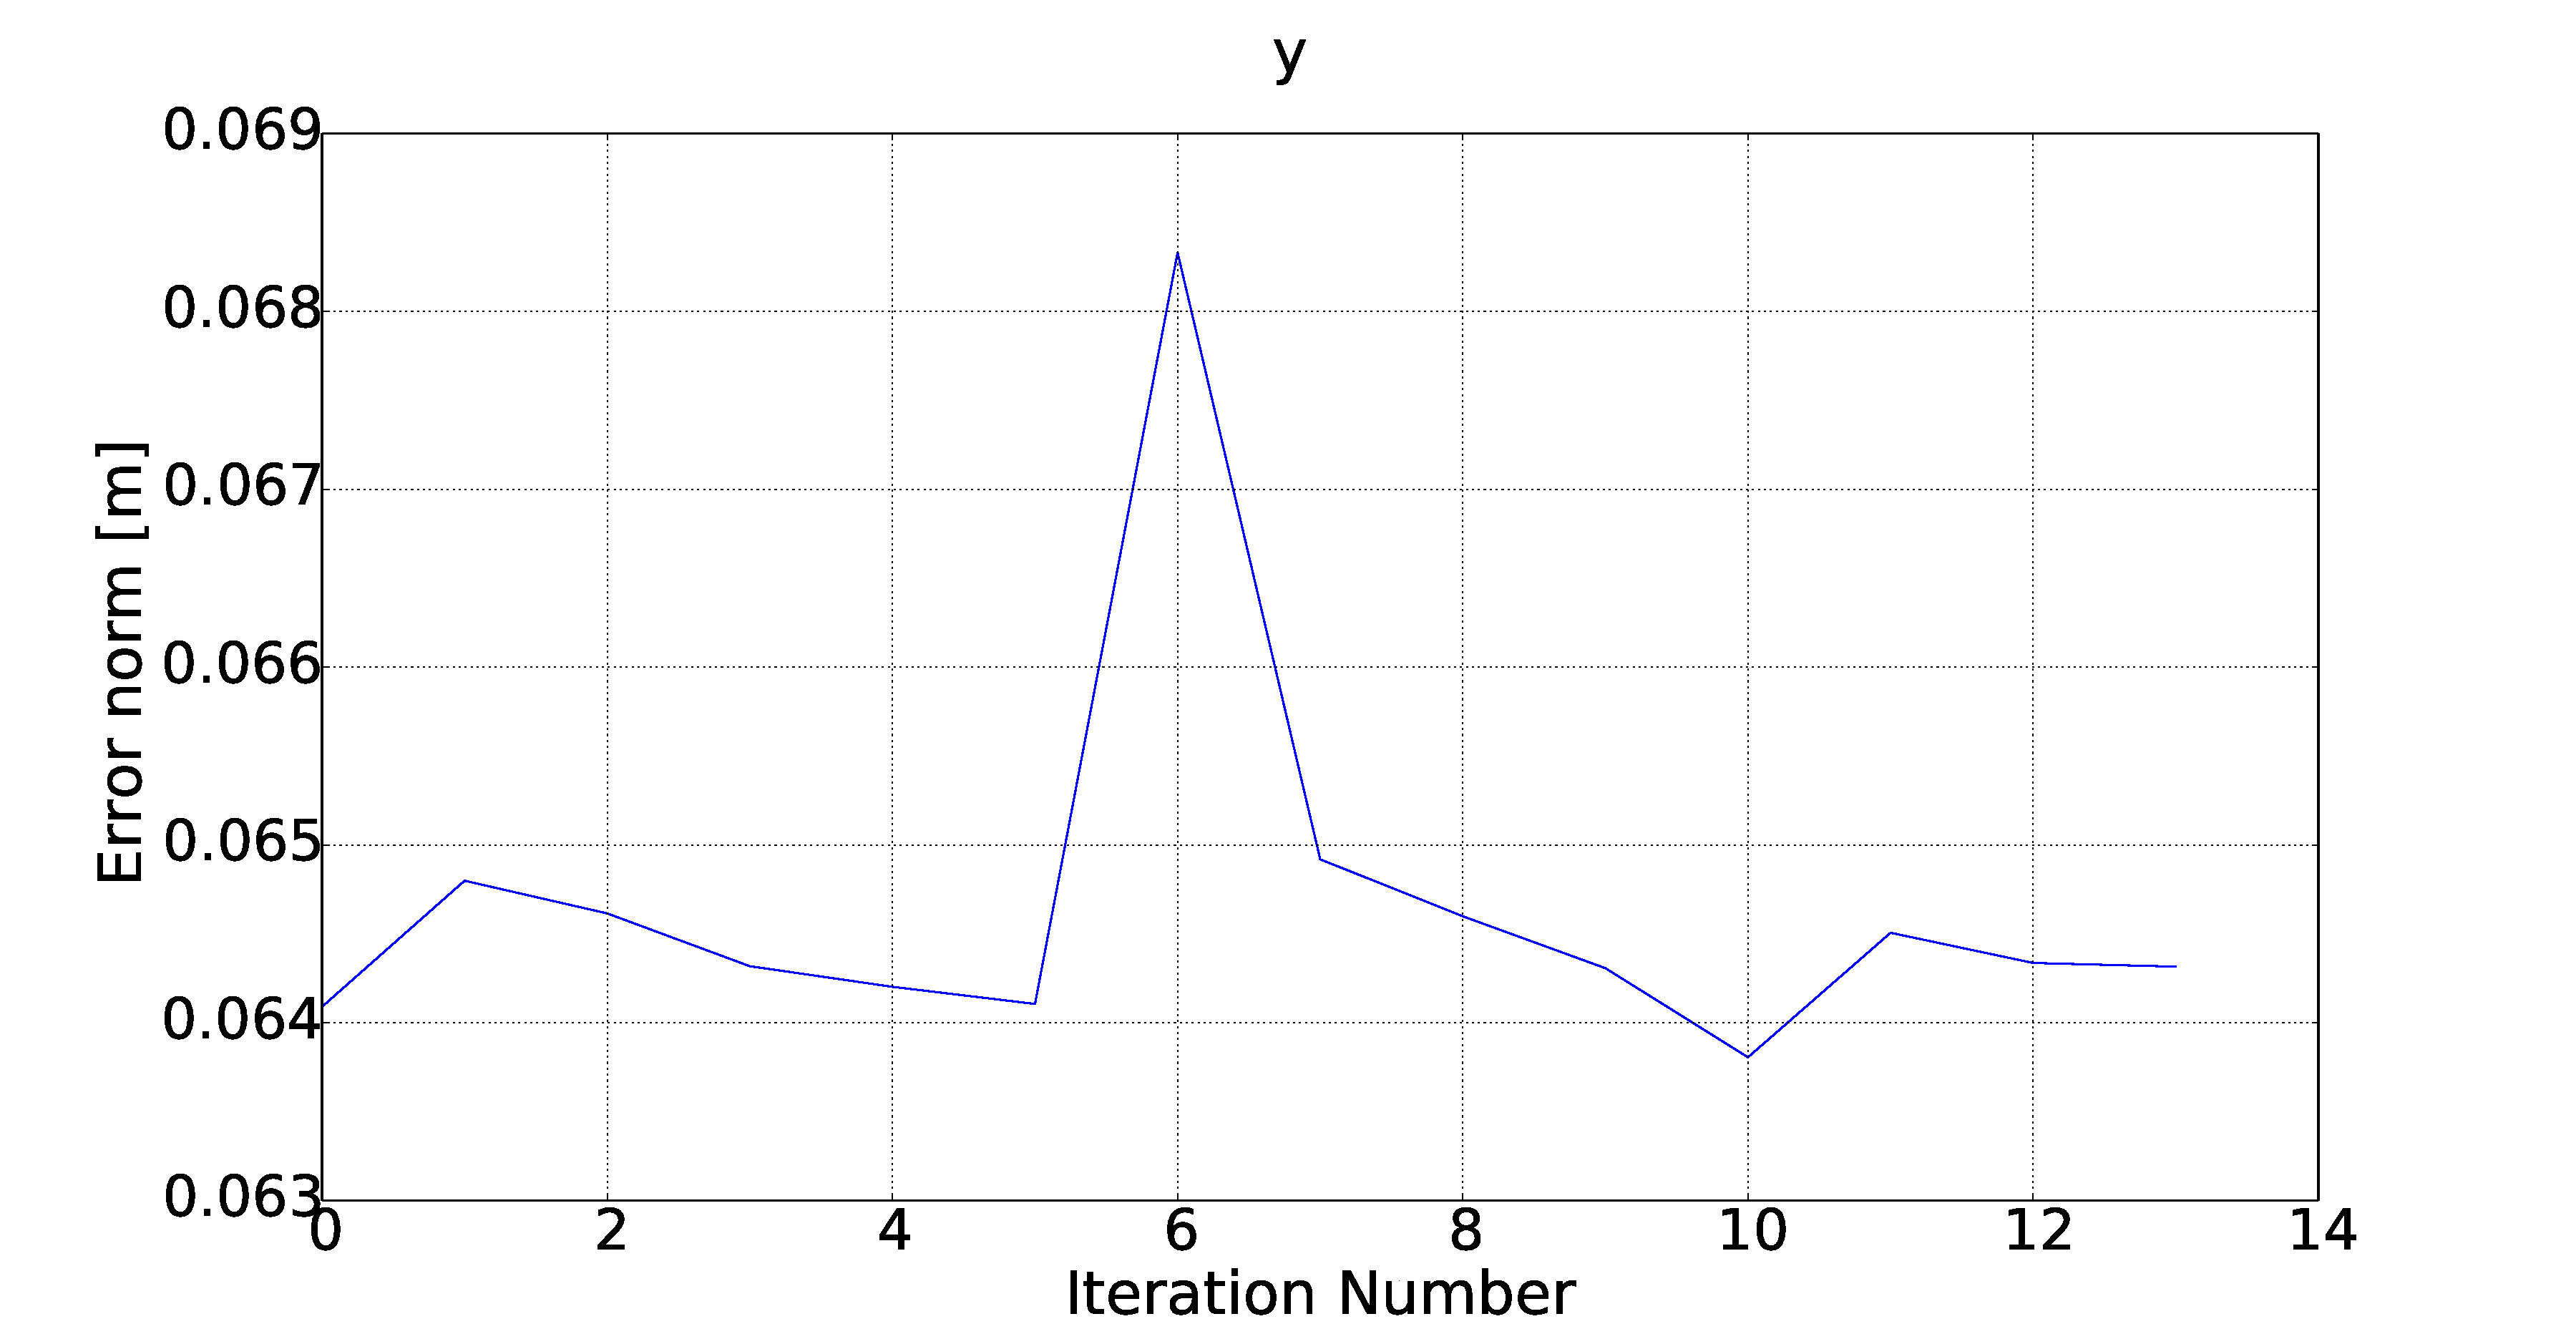
\includegraphics[width=\textwidth]{figures/chapter3/err_y.pdf}
    \caption{Error convergence in the $y$ dimension [m].}
\label{fig:err-convergence-y}
  \end{subfigure}
~
\begin{subfigure}{0.45\textwidth}
    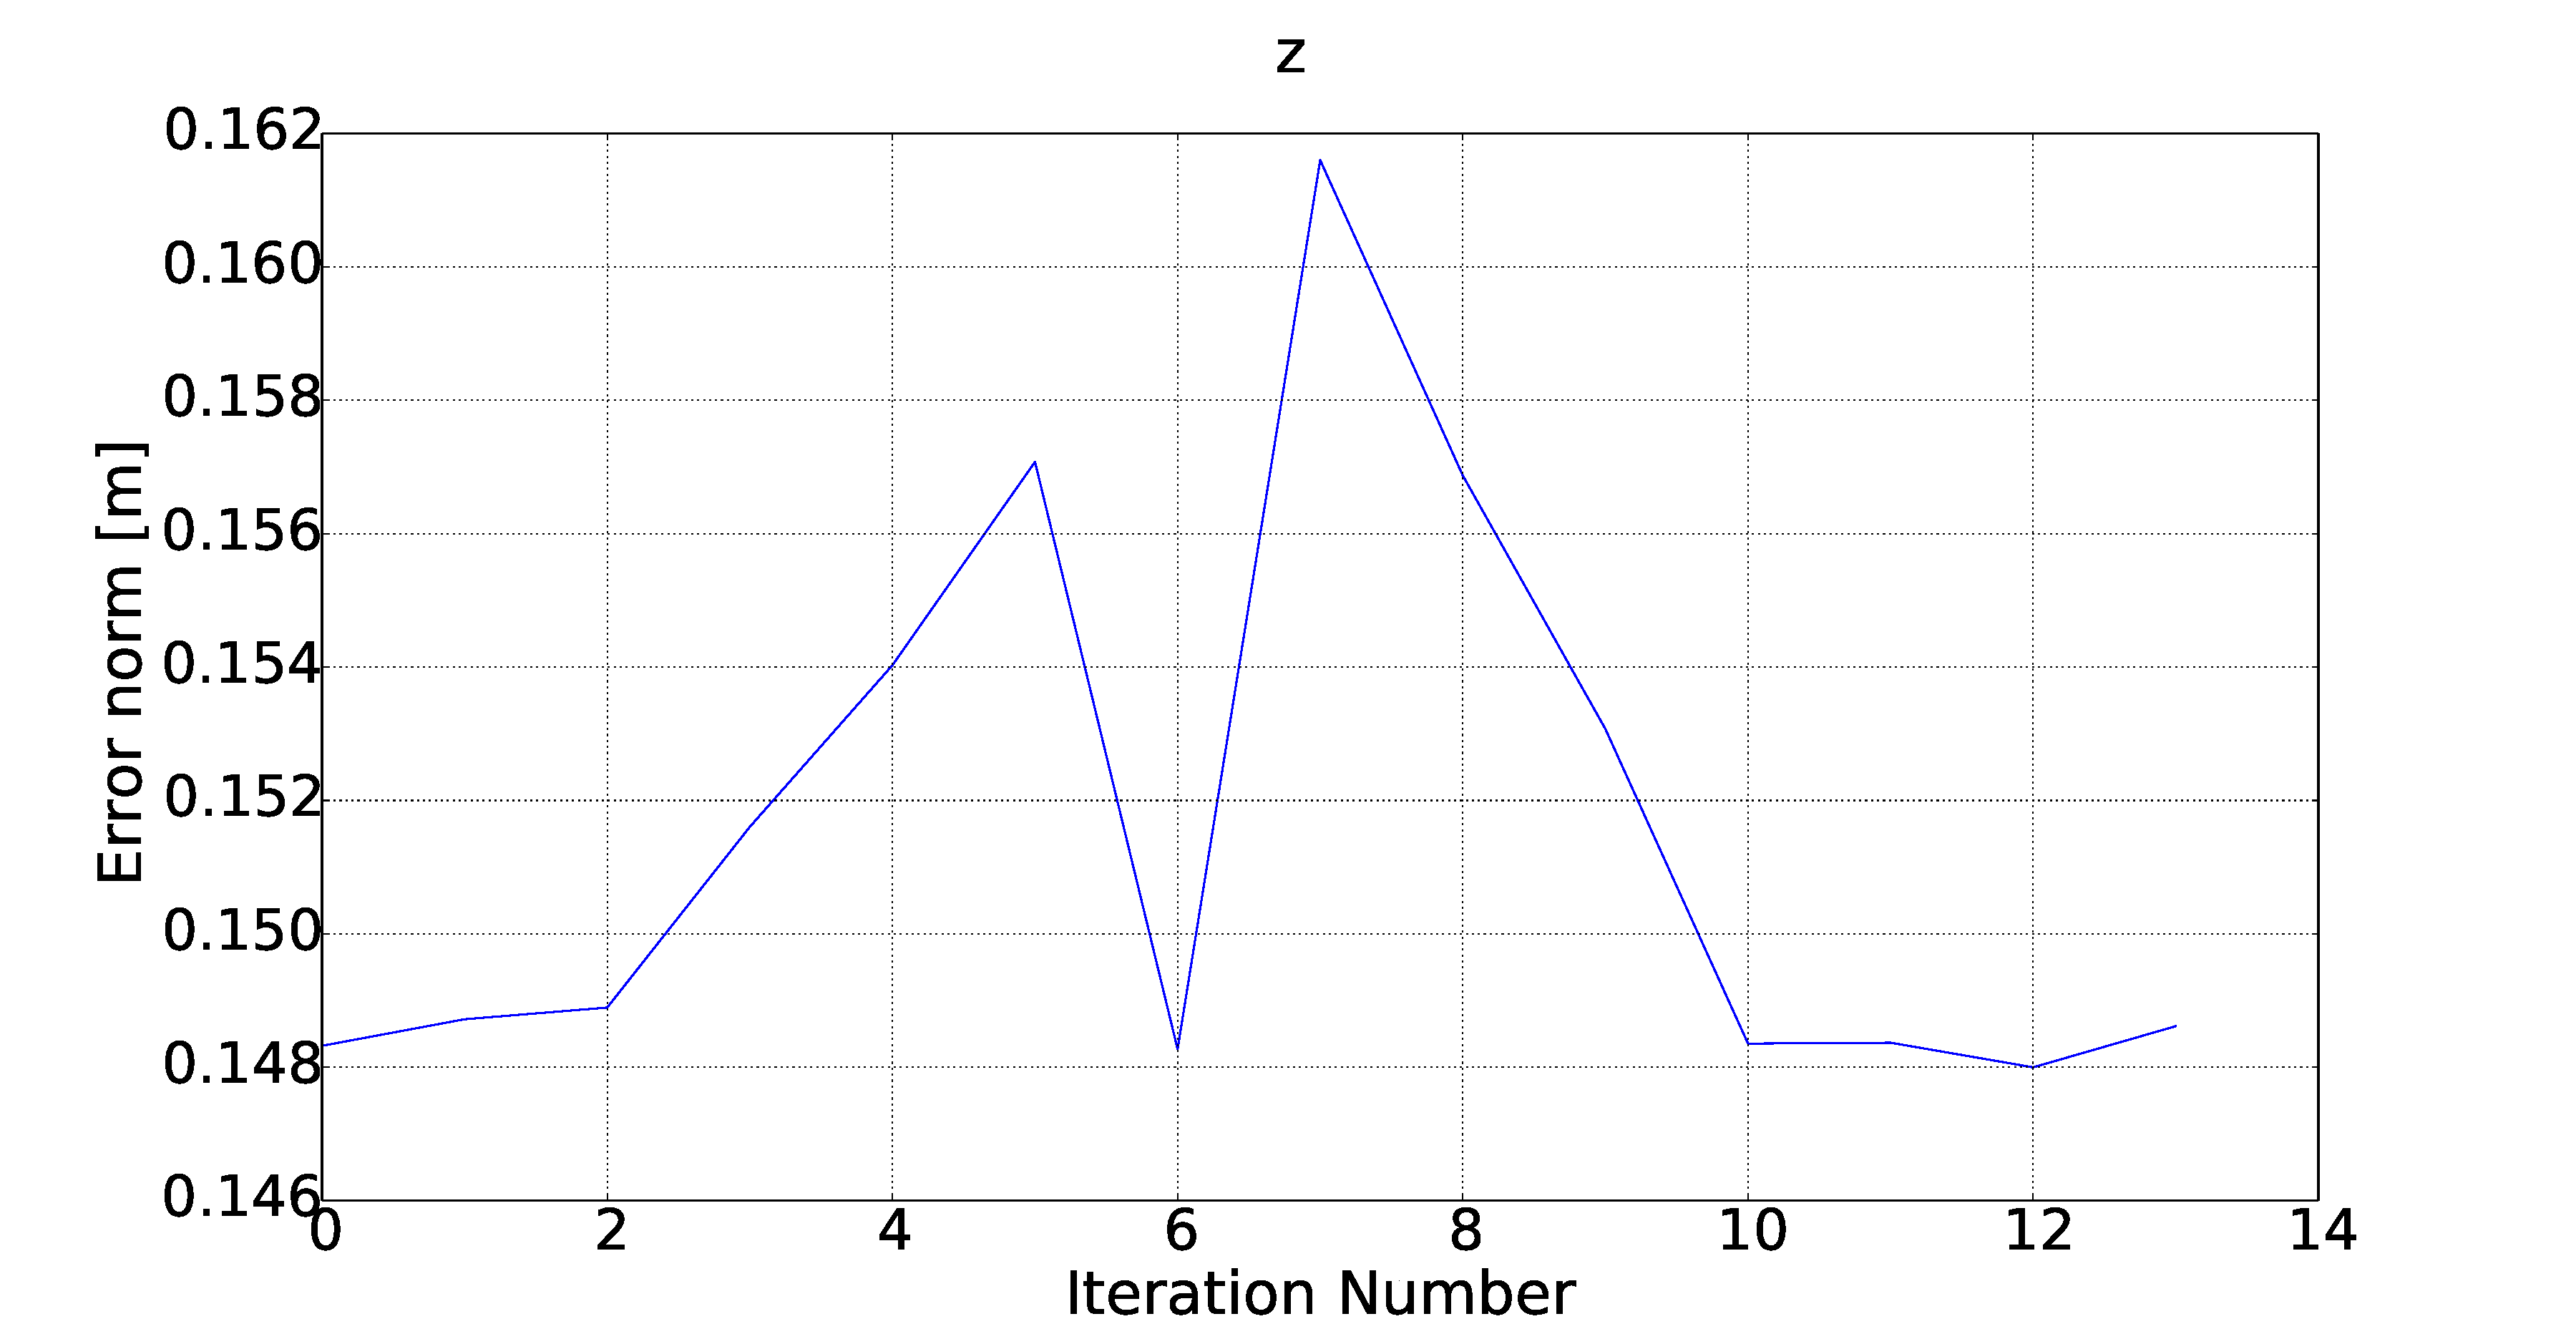
\includegraphics[width=\textwidth]{figures/chapter3/err_z.pdf}
    \caption{Error convergence in the $z$ dimension [m].}
\label{fig:err-convergence-z}
  \end{subfigure}
~
  \begin{subfigure}{0.45\textwidth}
    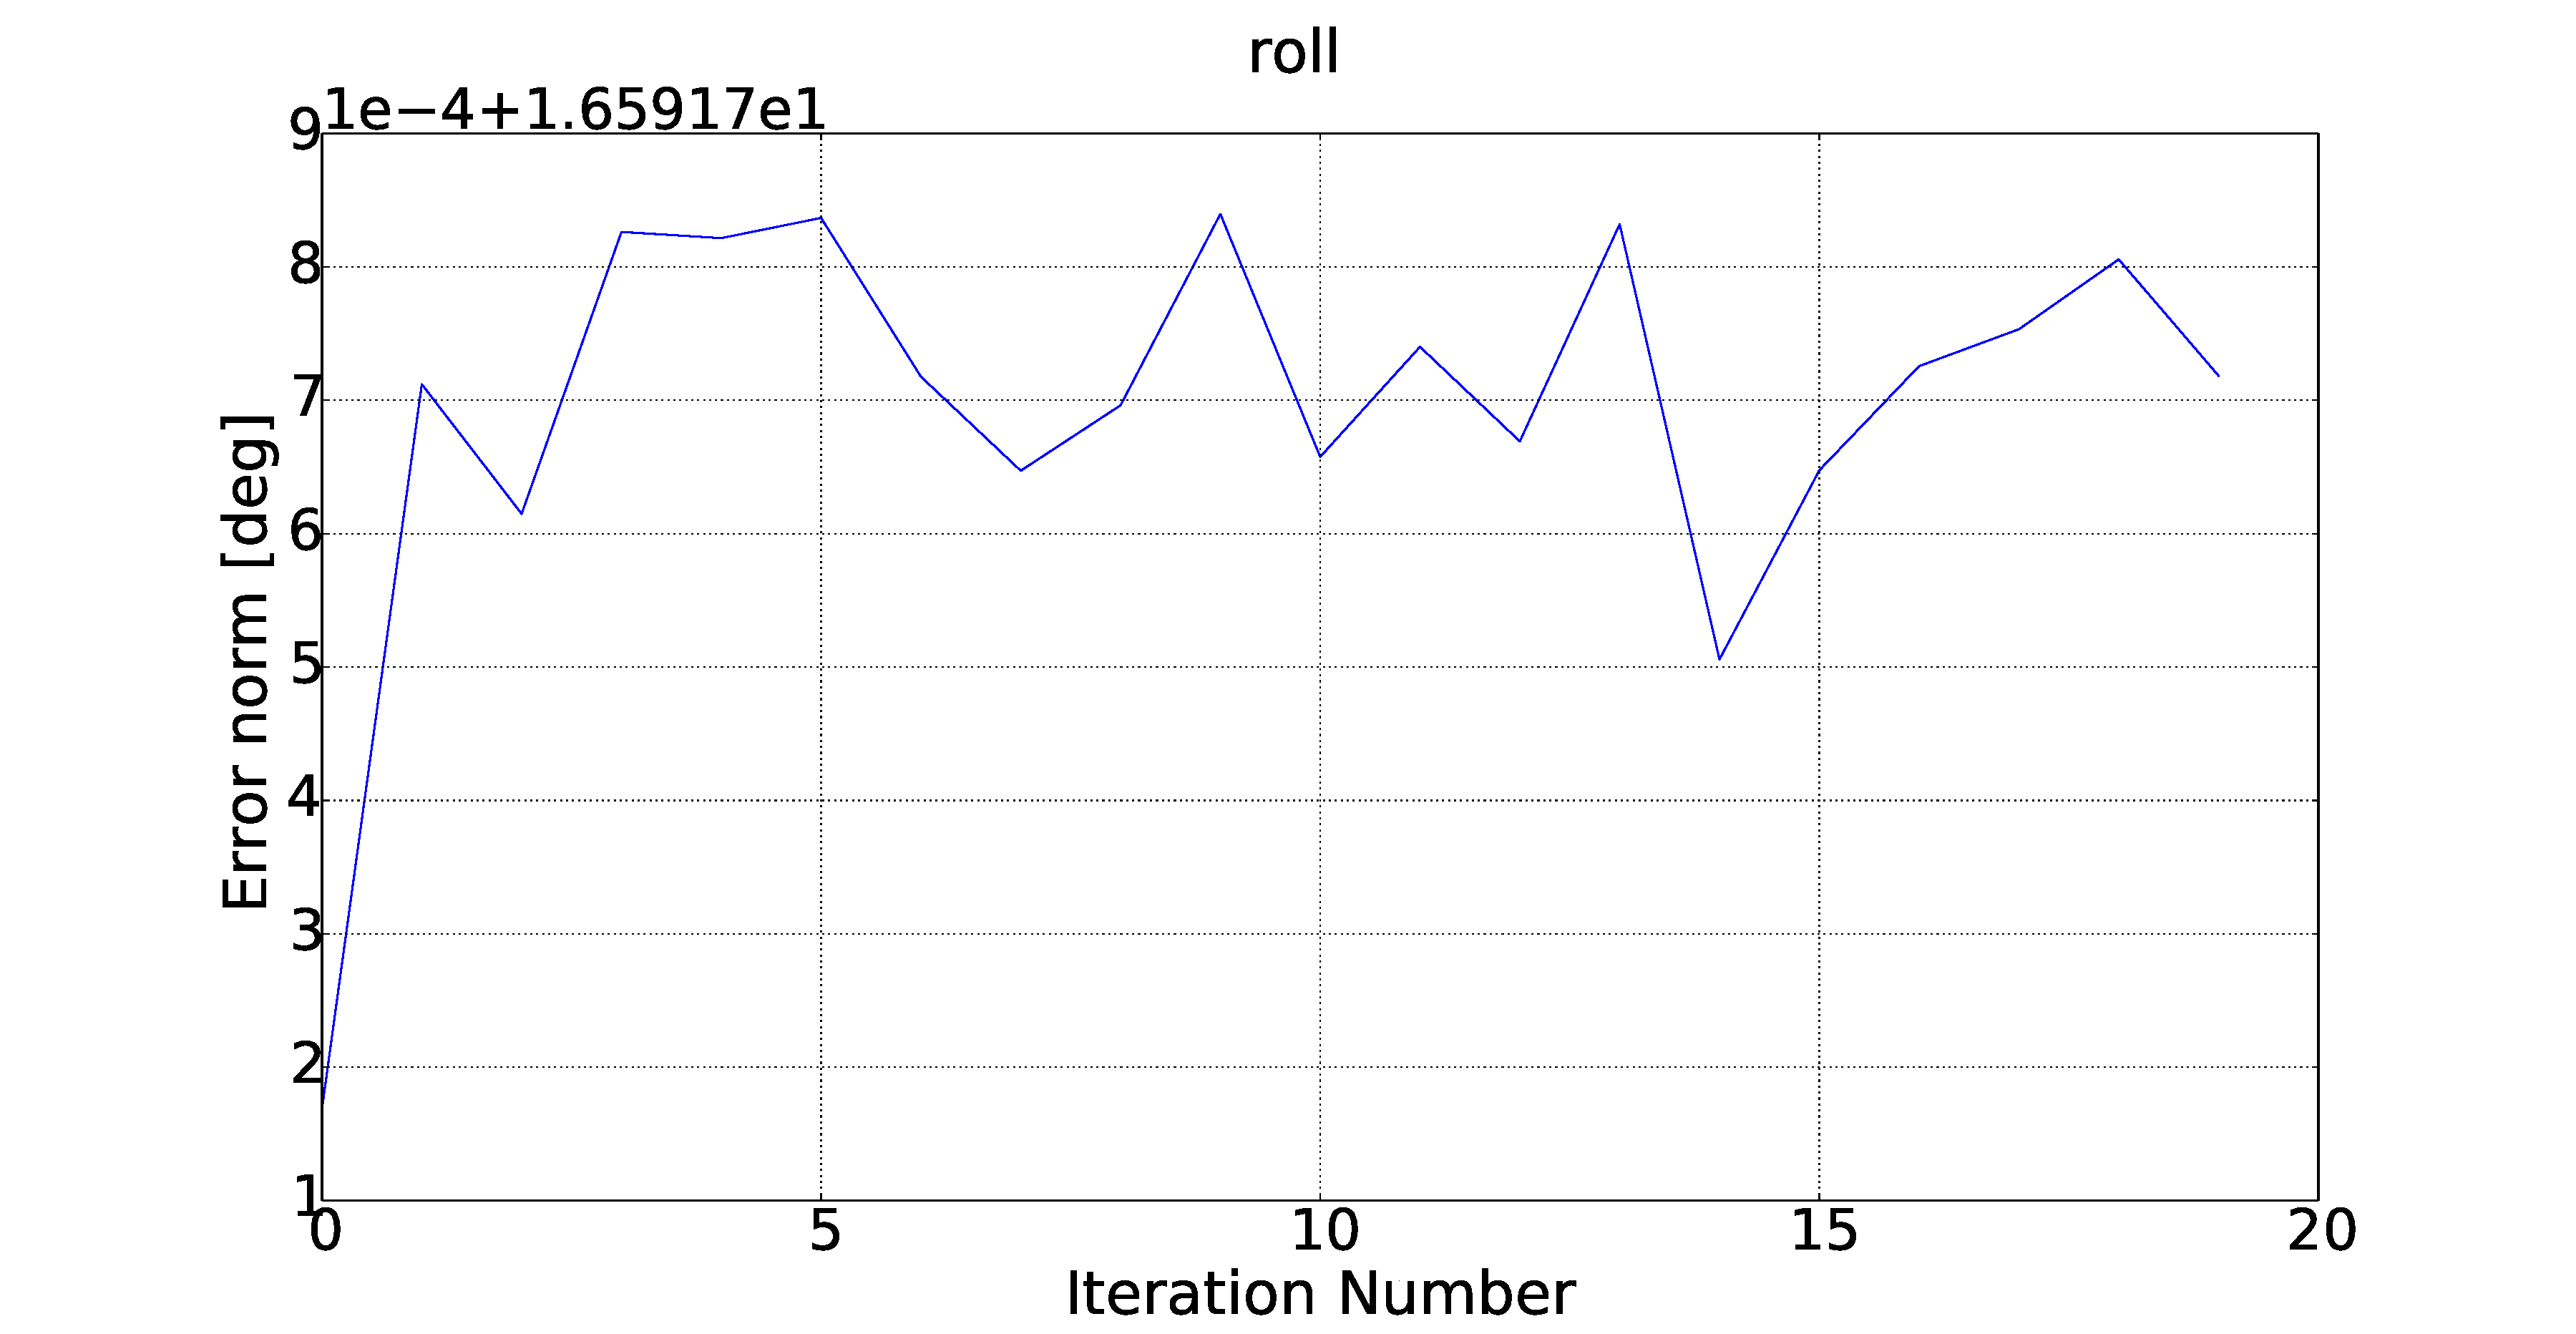
\includegraphics[width=\textwidth]{figures/chapter3/err_roll.pdf}
    \caption{Error convergence in the $\theta$ dimension [degrees].}
\label{fig:err-convergence-roll}
  \end{subfigure}
~
  \begin{subfigure}{0.45\textwidth}
    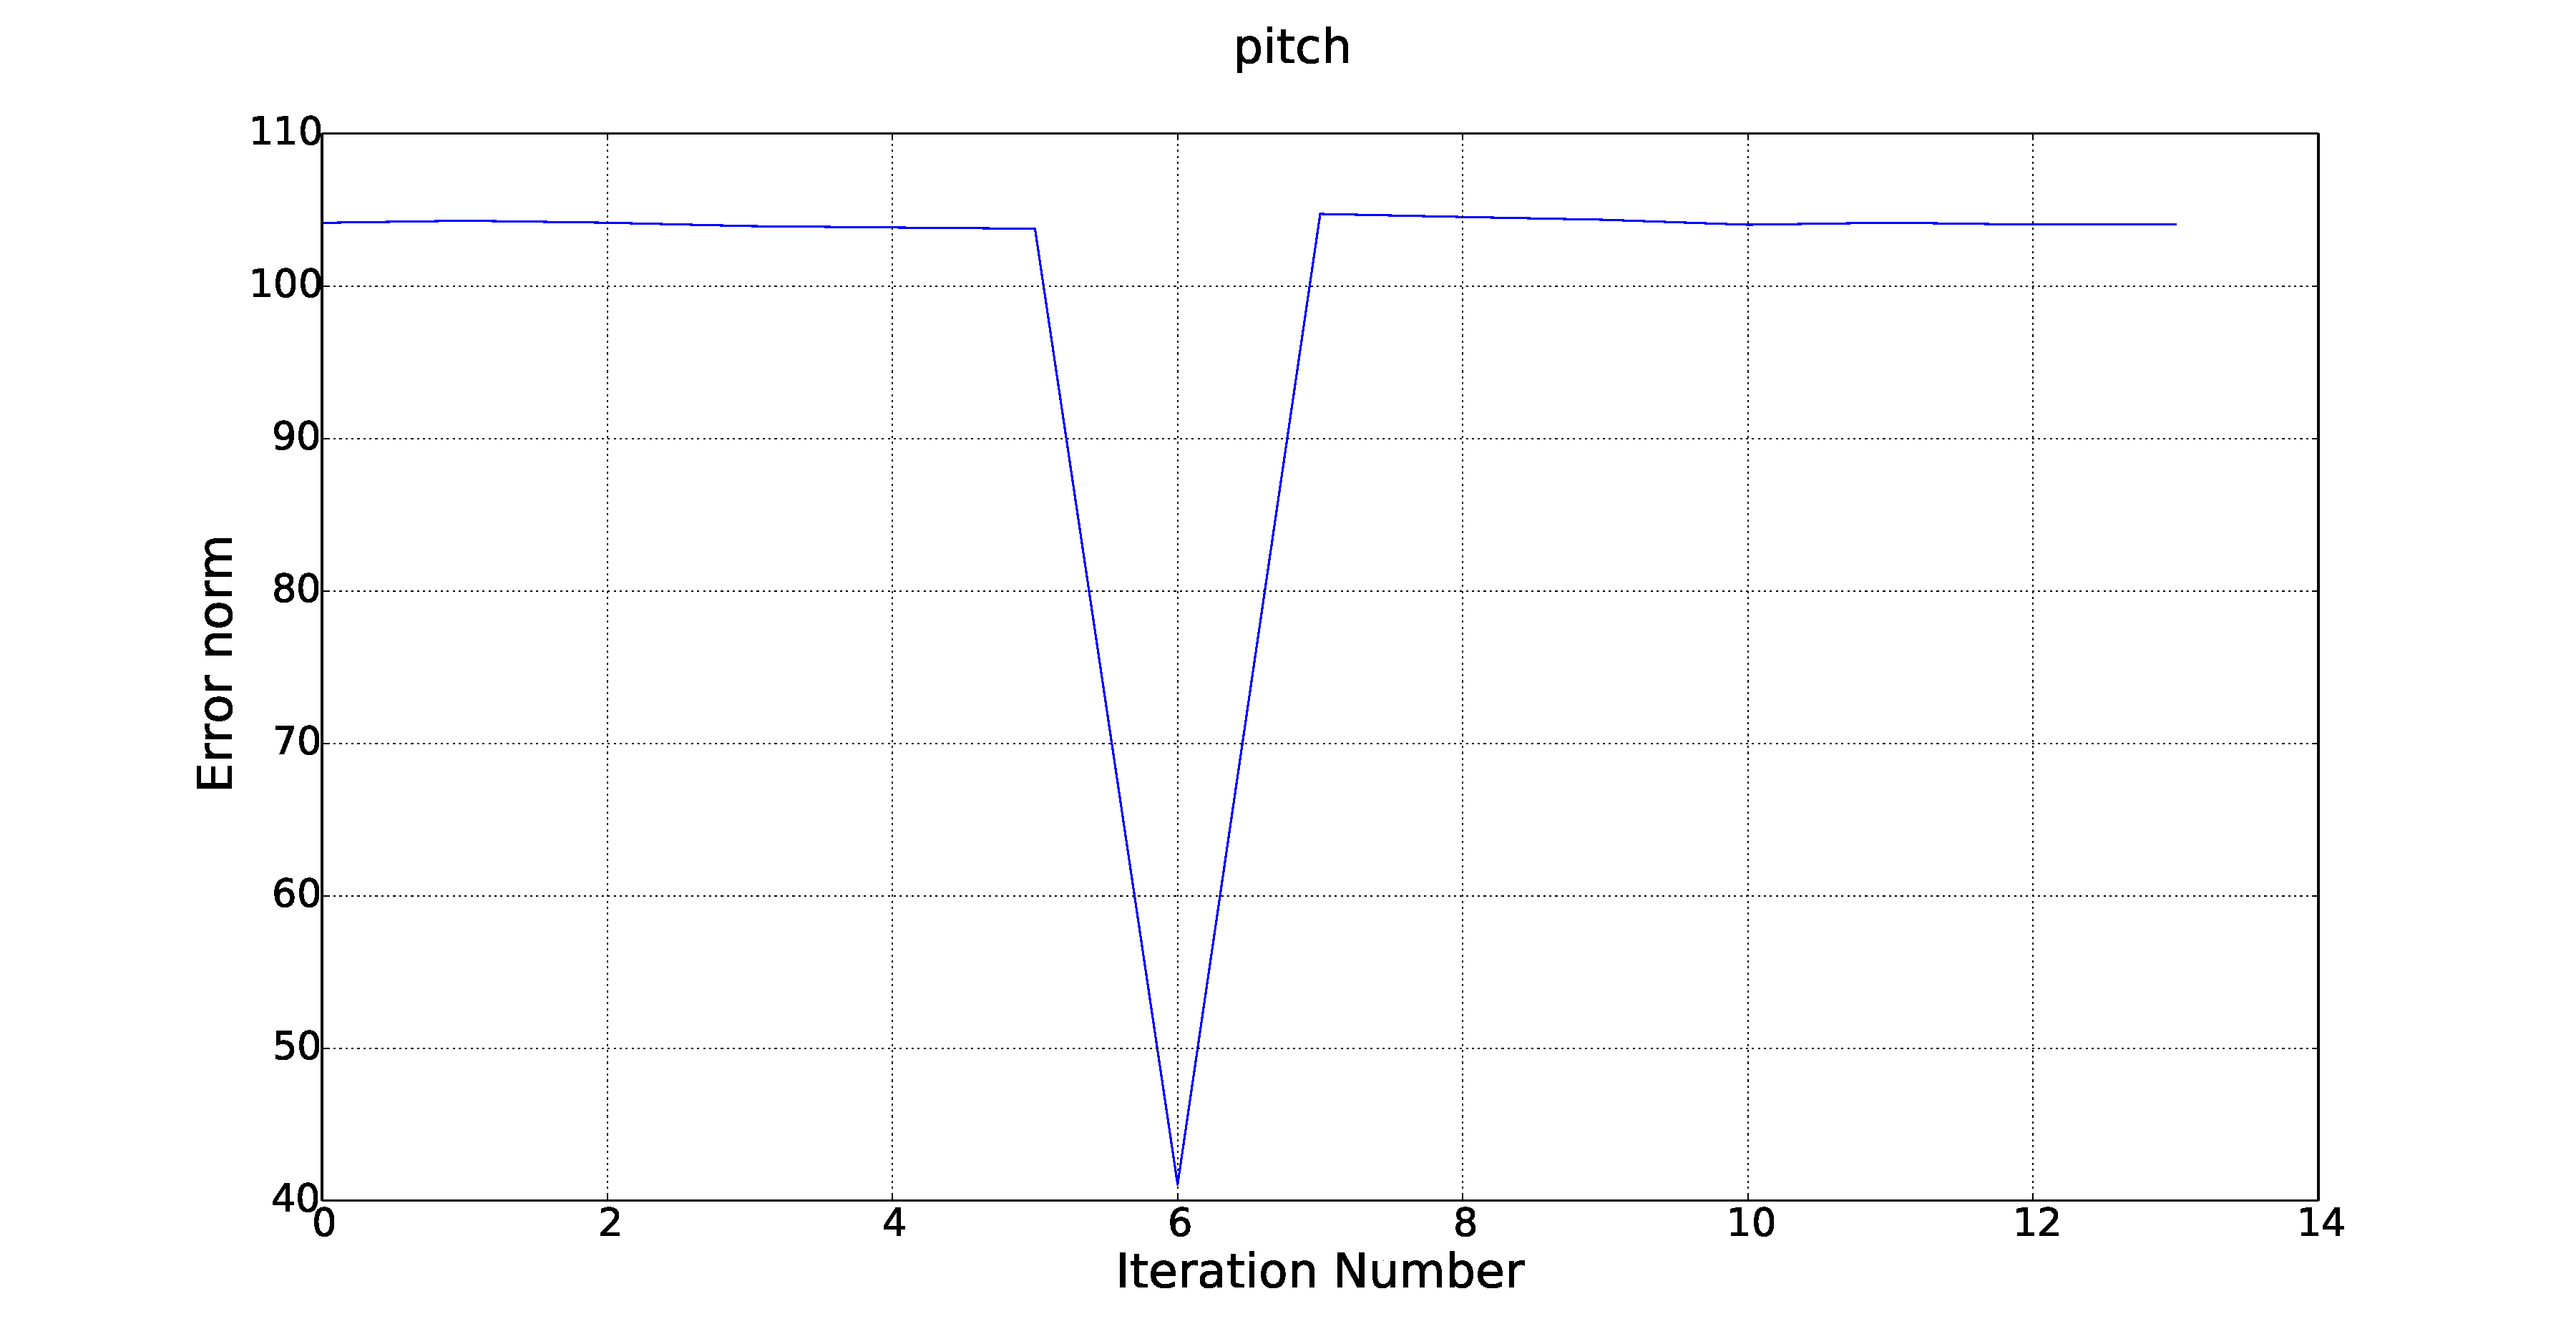
\includegraphics[width=\textwidth]{figures/chapter3/err_pitch.pdf}
    \caption{Error convergence in the $\phi$ dimension [degrees].}
\label{fig:err-convergence-pitch}
  \end{subfigure}
~
  \begin{subfigure}{0.45\textwidth}
    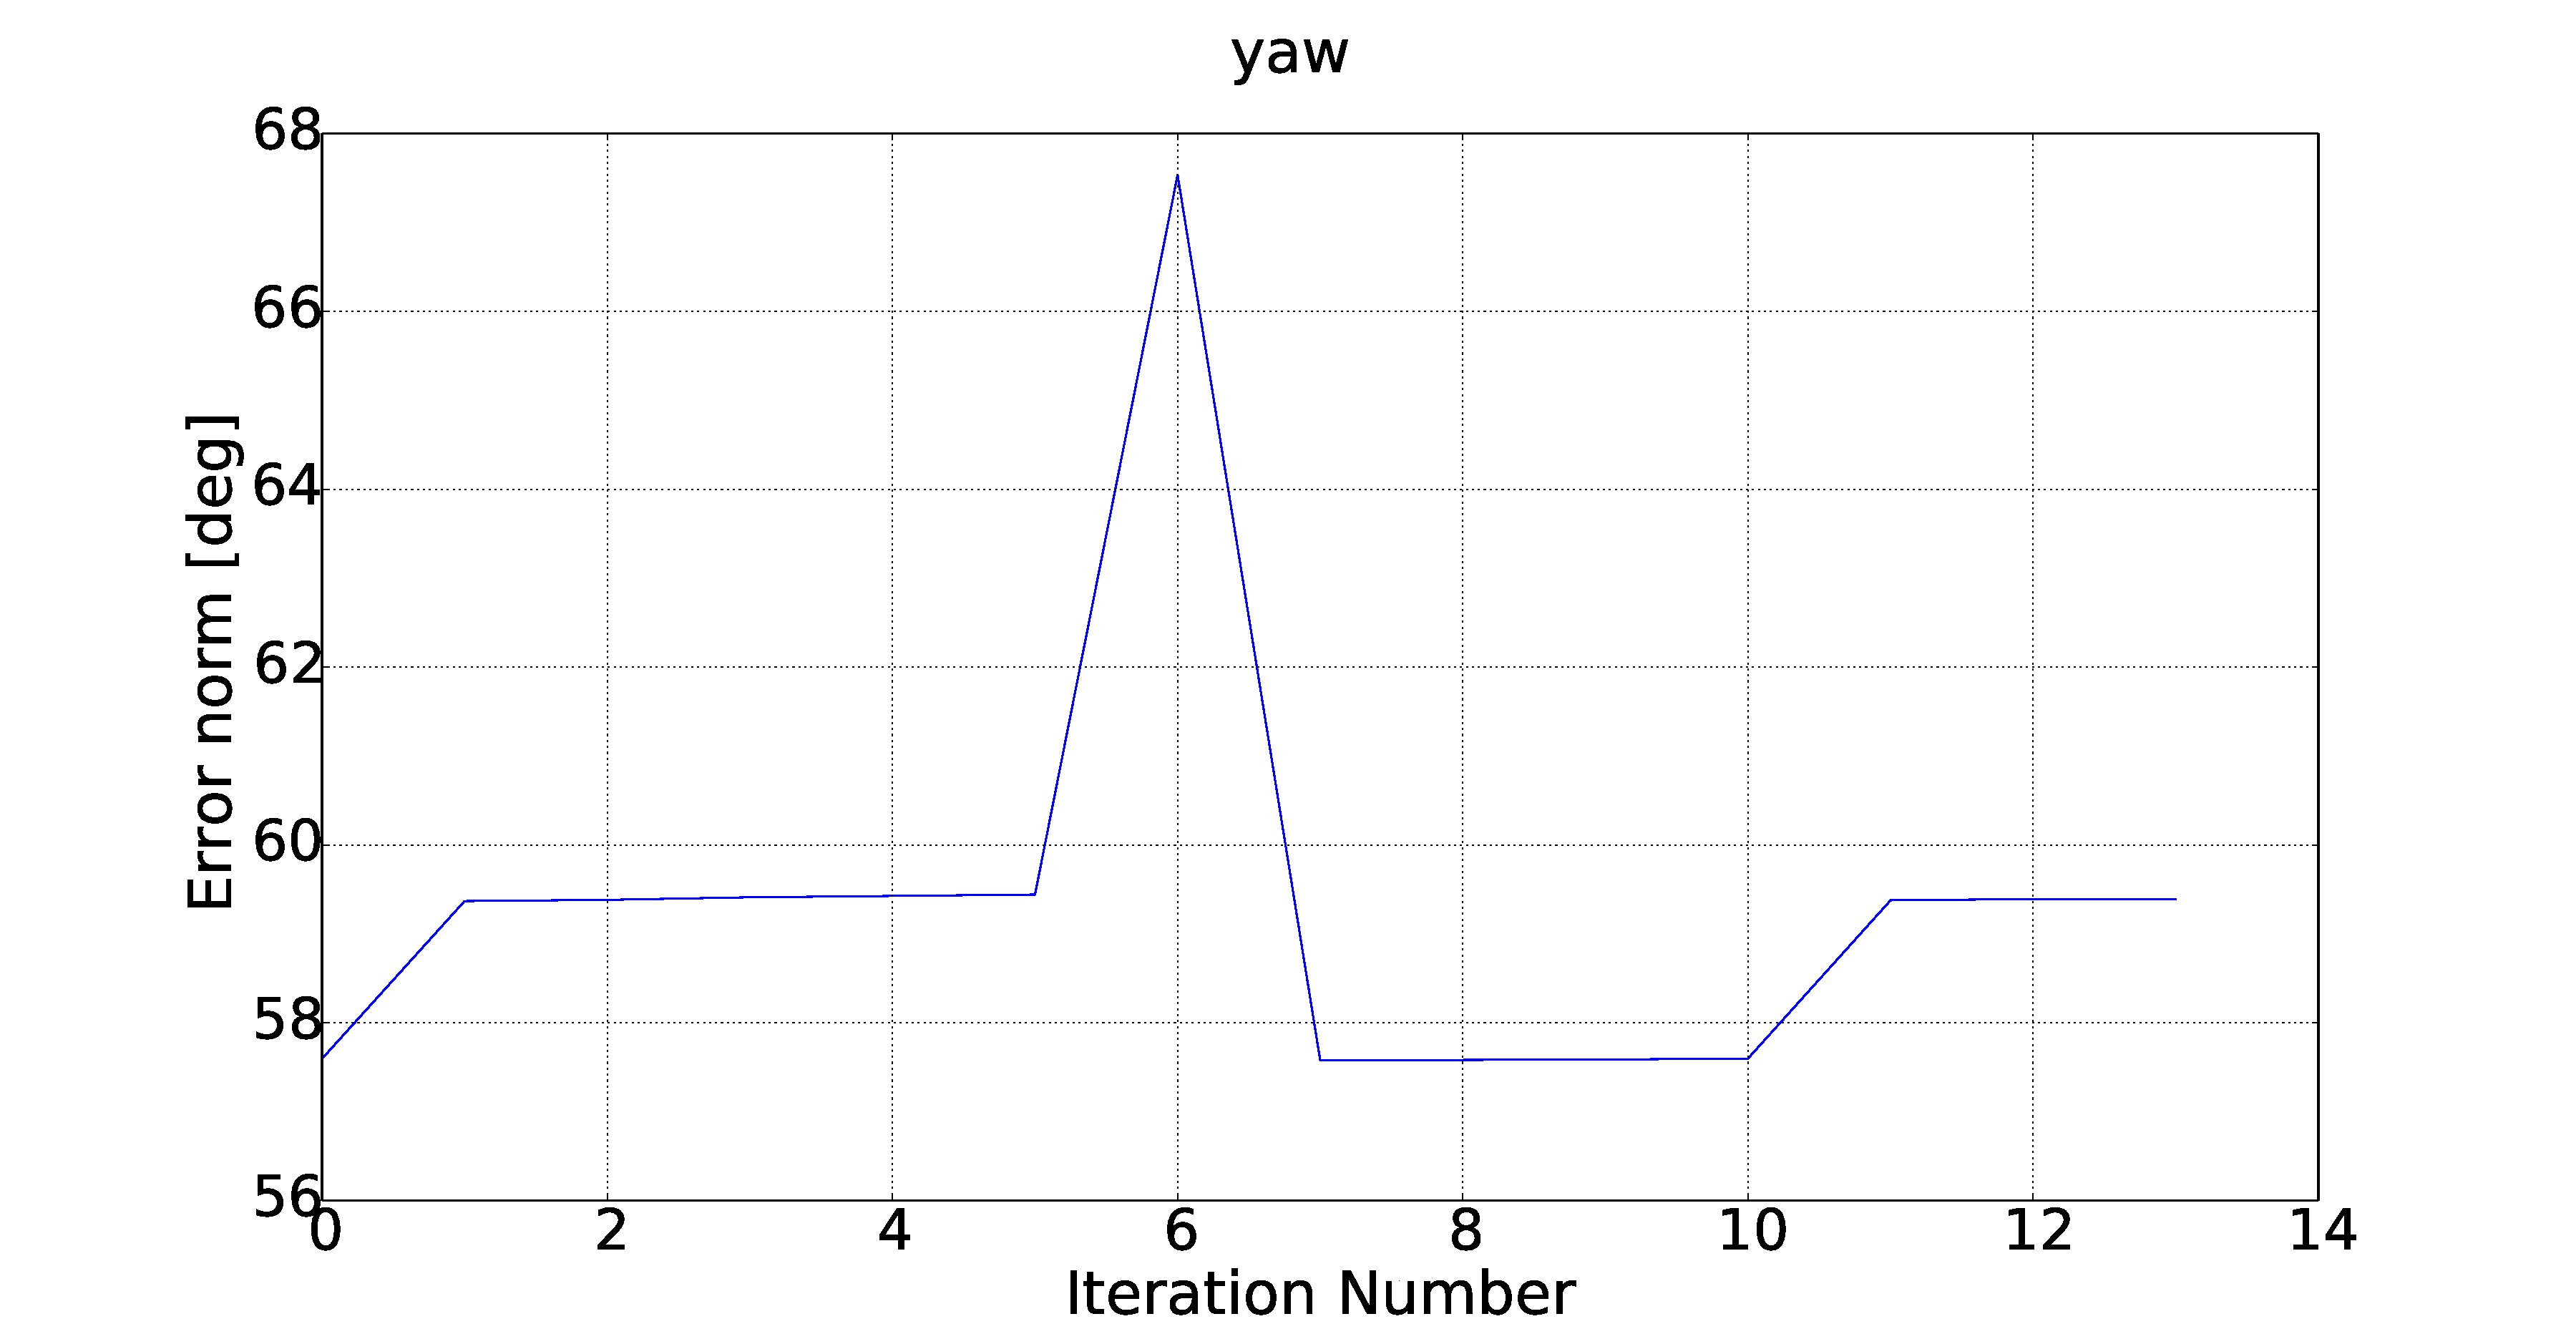
\includegraphics[width=\textwidth]{figures/chapter3/err_yaw.pdf}
    \caption{Error convergence in the $\psi$ dimension [degrees].}
\label{fig:err-convergence-psi}
  \end{subfigure}
  \caption{Plots showing the error in each dimension during for each iteration of the error minimisation procedure.}
  \label{fig:err-convergence}
\end{figure*}

The graphs in Figure~\ref{fig:err-convergence} show that the error gets reduced in the $x$ and $z$ dimensions, while it gets worse in the $y$ and rotation dimensions. Since the optimisation procedure is based on the error in the translation vector, it is not surprising that the rotation error grows. However, the $y$ dimension error growing is somewhat surprising.  %These figures show that the error hovers around 0 after only a few iterations, but does not fully converge. This may warrant some investigation, but it is suspected that the focal length step sizes are too large and must be adapted between iterations. This will be implemented in later versions.

Upon closer inspection, it can be seen that of the three translation vectors, the $y$ dimension has the lowest total error. Since all three vectors carry the same importance weighting for optimisation, it is inevitable that the $x$ and $z$ dimension's errors get lowered at the cost of the $y$ dimension's accuracy. 

\subsection{Test for Normality}
\label{sec:err-norm-test}

To check if $\bm{\epsilon}$ is indeed normally distributed as assumed in Equation~\ref{eq:offset}, a frequency histogram of the error matrix $\epsilon$ in all six dimensions are plotted along with a normal distribution drawn using each dimension's mean and standard deviation. A $\chi^2$ test could also have been used. However, it was found that the sample size of the data set was too large and it is known that some skewness in the data can have a large impact on the $\chi^2$ probability estimate. Therefore, a graphical approach was taken to determining if the errors are normally distributed around 0.0. 

Figure~\ref{fig:err-norm} shows the histogram plots of the errors in the six dimensions. A normal distribution, using the averages and standard deviations from the data set, are superimposed to illustrate the normal distribution of the data.

%\begin{figure*}
  %\begin{subfigure}{0.45\textwidth}
     %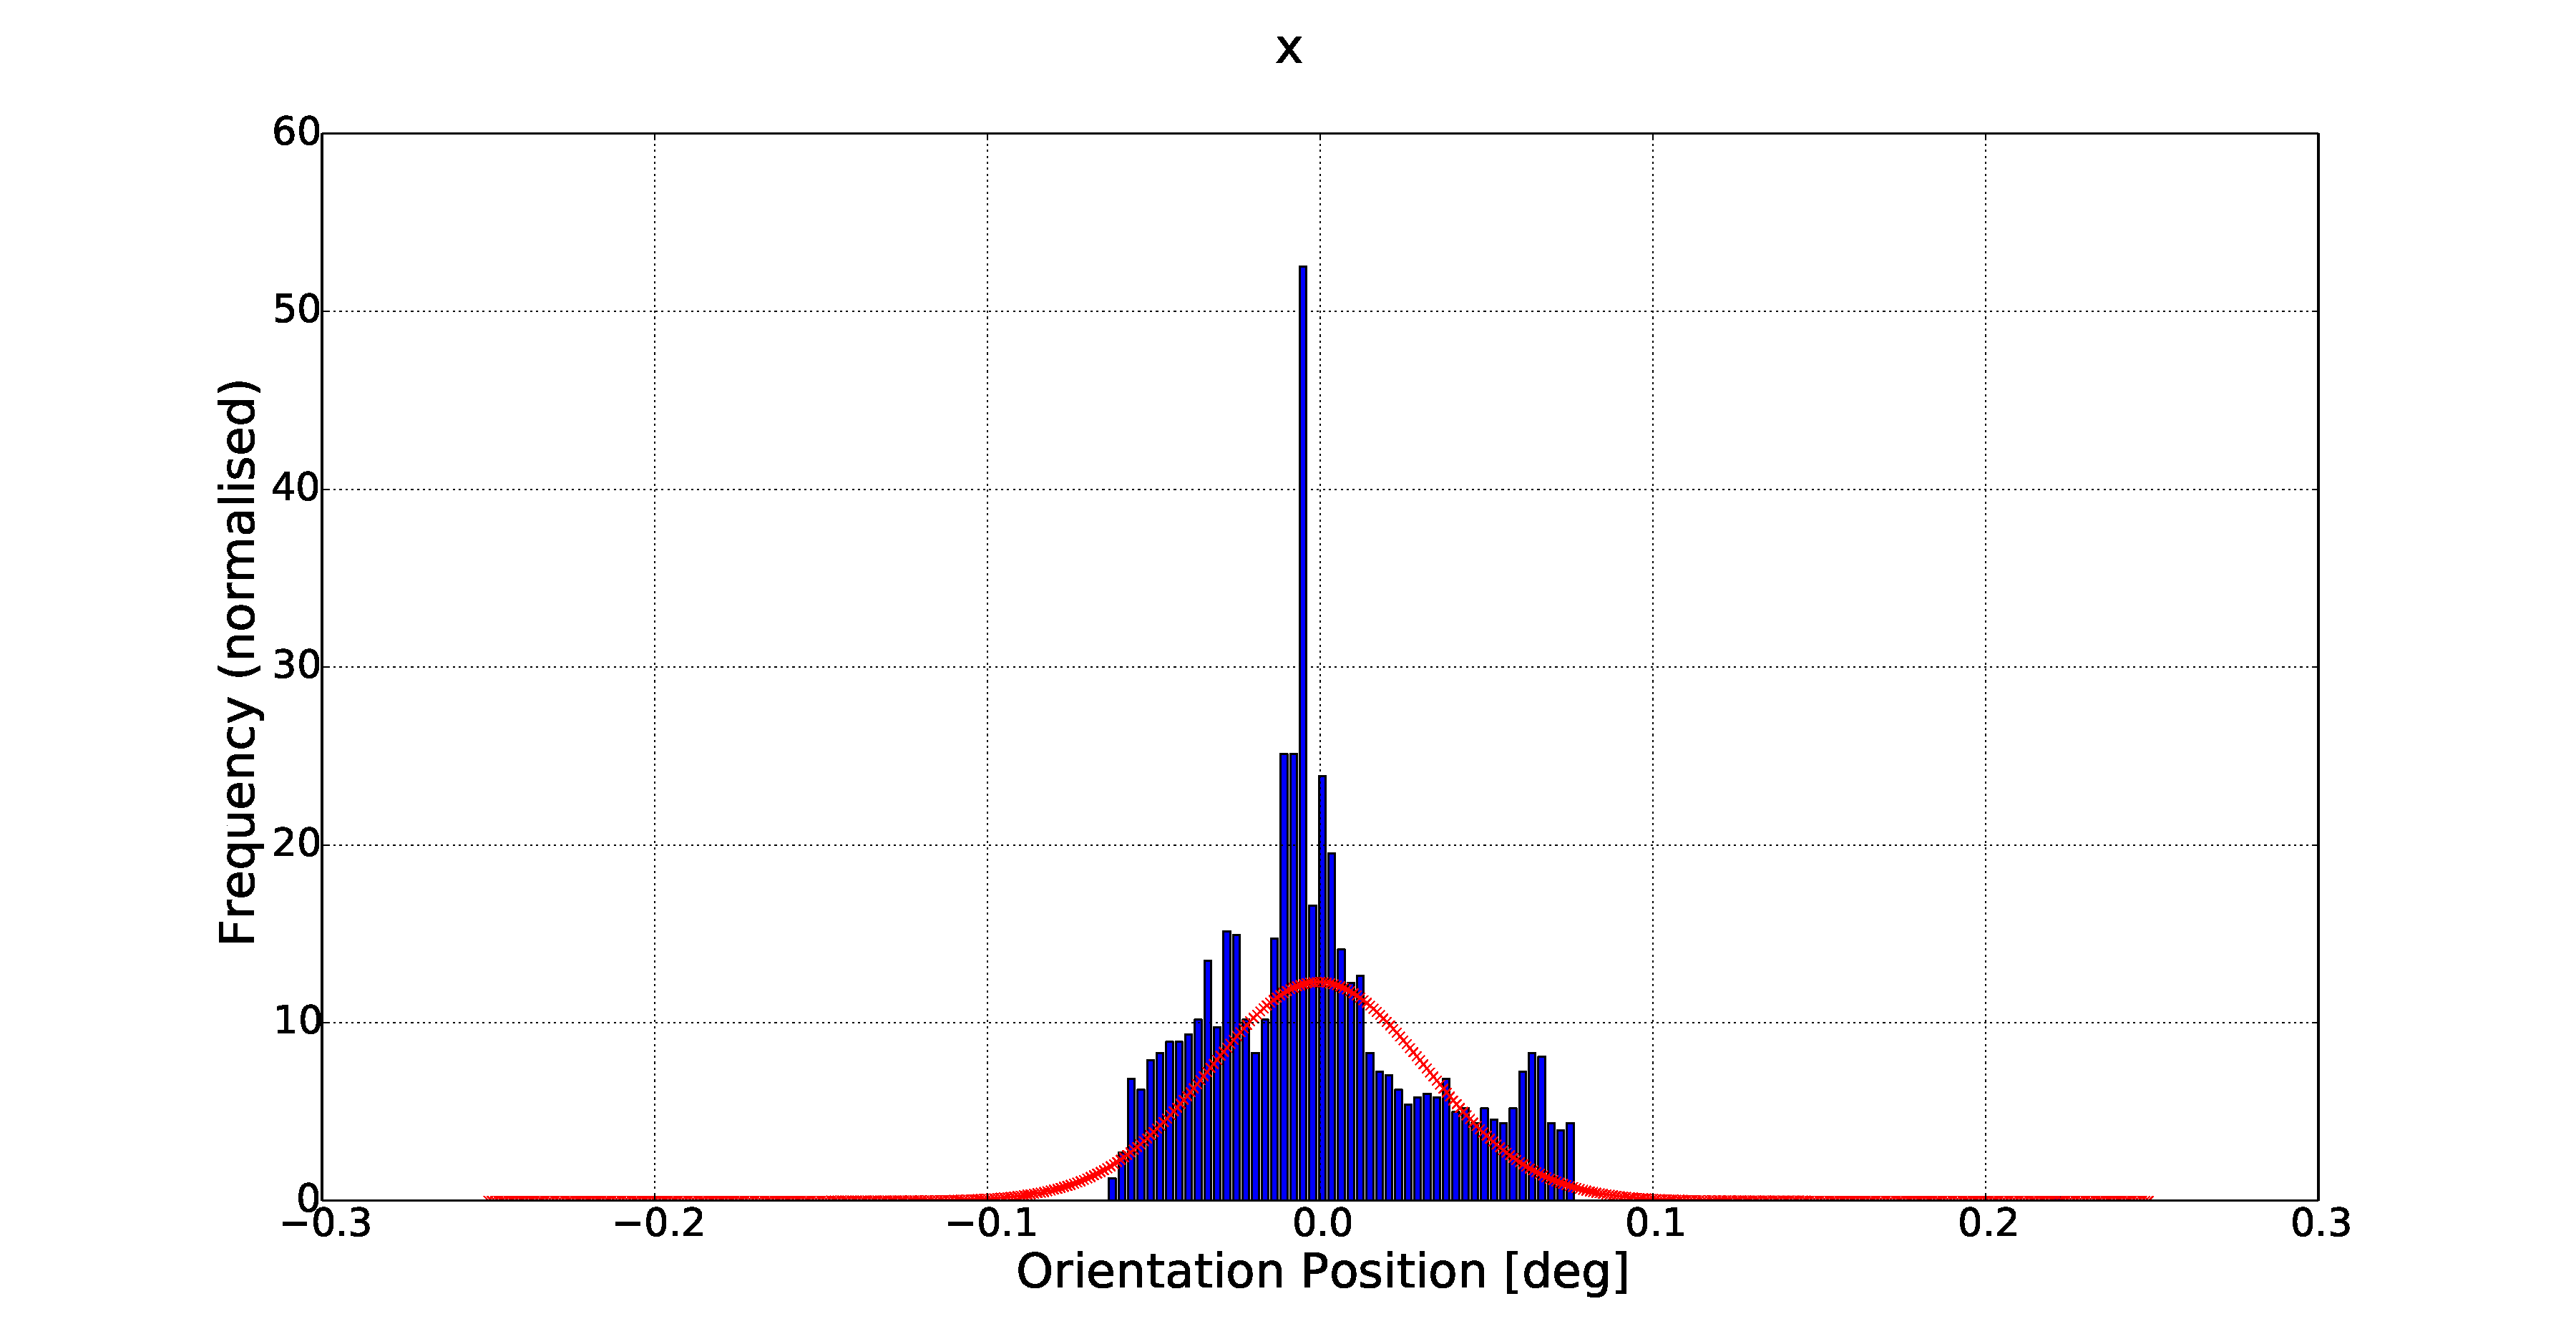
\includegraphics[clip, trim = 150 50 155 0, width=\textwidth]{figures/chapter3/norm_x.pdf}
     %\caption{Histogram of the error in the $x$ dimension with a mean of $-5.17\mu$m and a standard deviation of 293mm.}
  %\label{fig:norm-x}
  %\end{subfigure}
%~
  %\begin{subfigure}{0.45\textwidth}
     %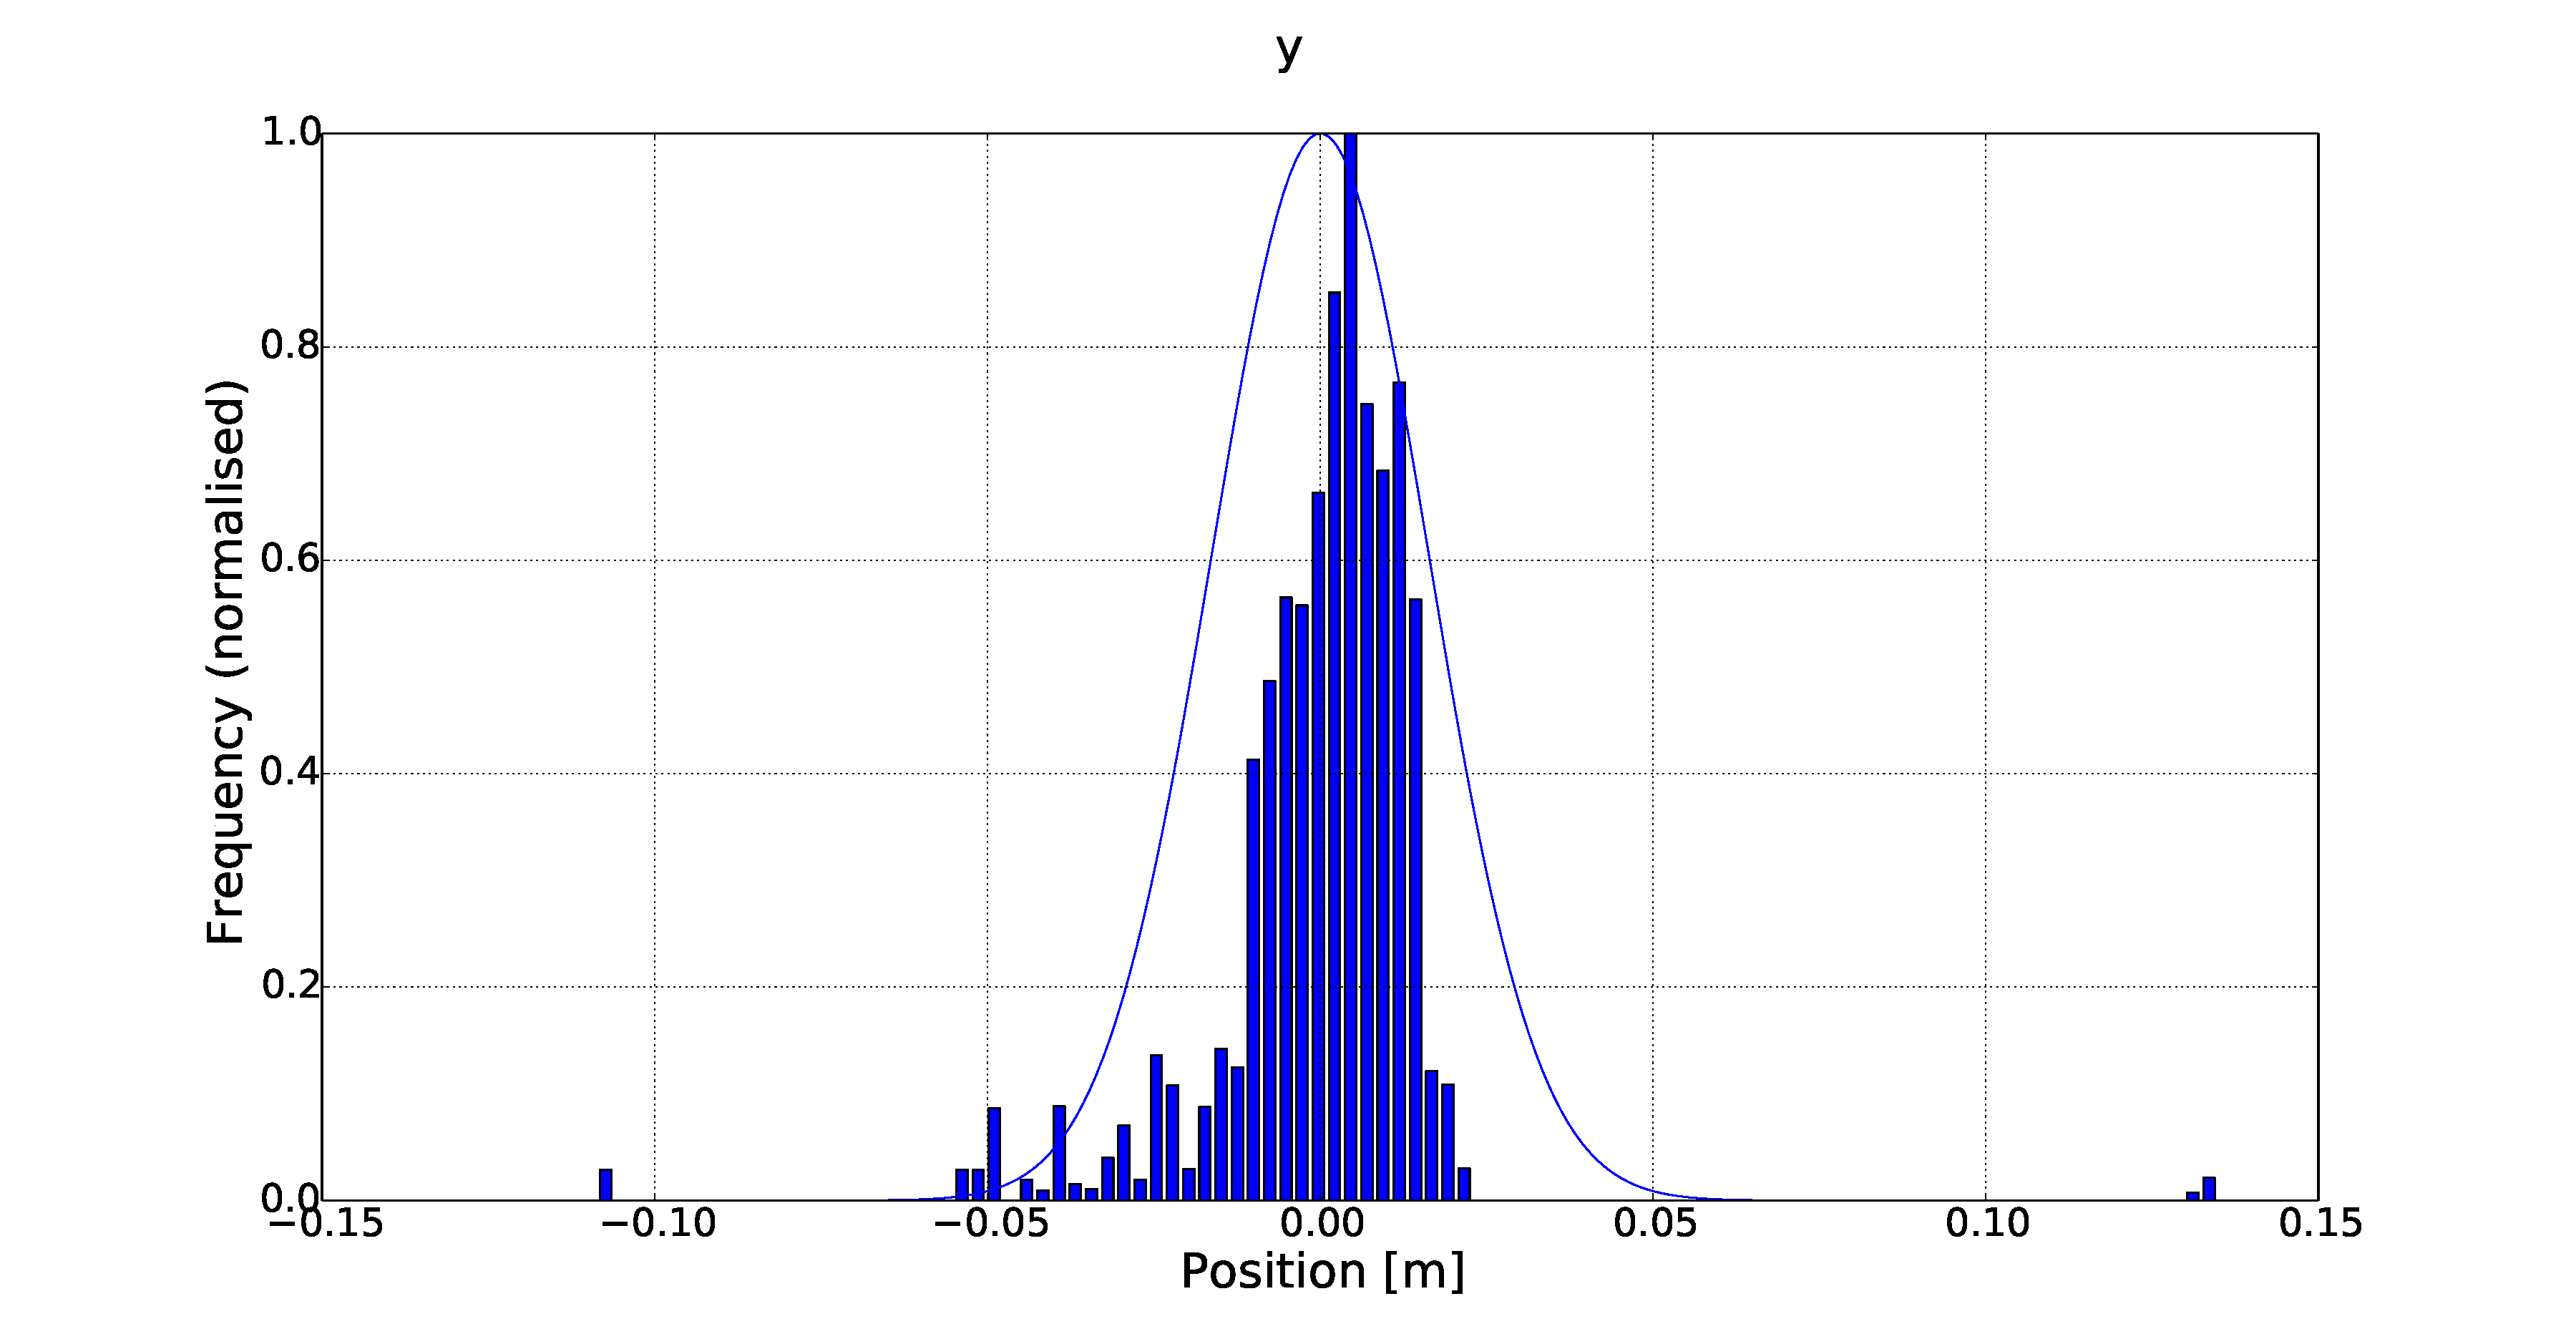
\includegraphics[clip, trim = 150 50 155 0, width=\textwidth]{figures/chapter3/norm_y.pdf}
     %\caption{Histogram of the error in the $y$ dimension with a mean of $-20.2\mu$m and a standard deviation of 167mm.}
  %\label{fig:norm-y}
  %\end{subfigure}
%~
  %\begin{subfigure}{0.45\textwidth}
     %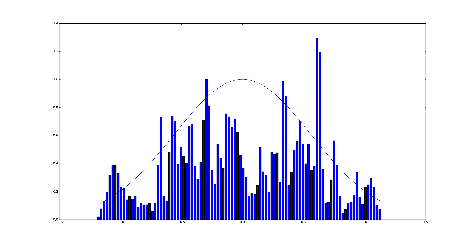
\includegraphics[clip, trim = 150 50 155 0, width=\textwidth]{figures/chapter3/norm_z.pdf}
     %\caption{Histogram of the error in the $z$ dimension with a mean of 1.17mm and a standard deviation of 560mm.}
  %\label{fig:norm-z}
  %\end{subfigure}
%~
  %\begin{subfigure}{0.45\textwidth}
     %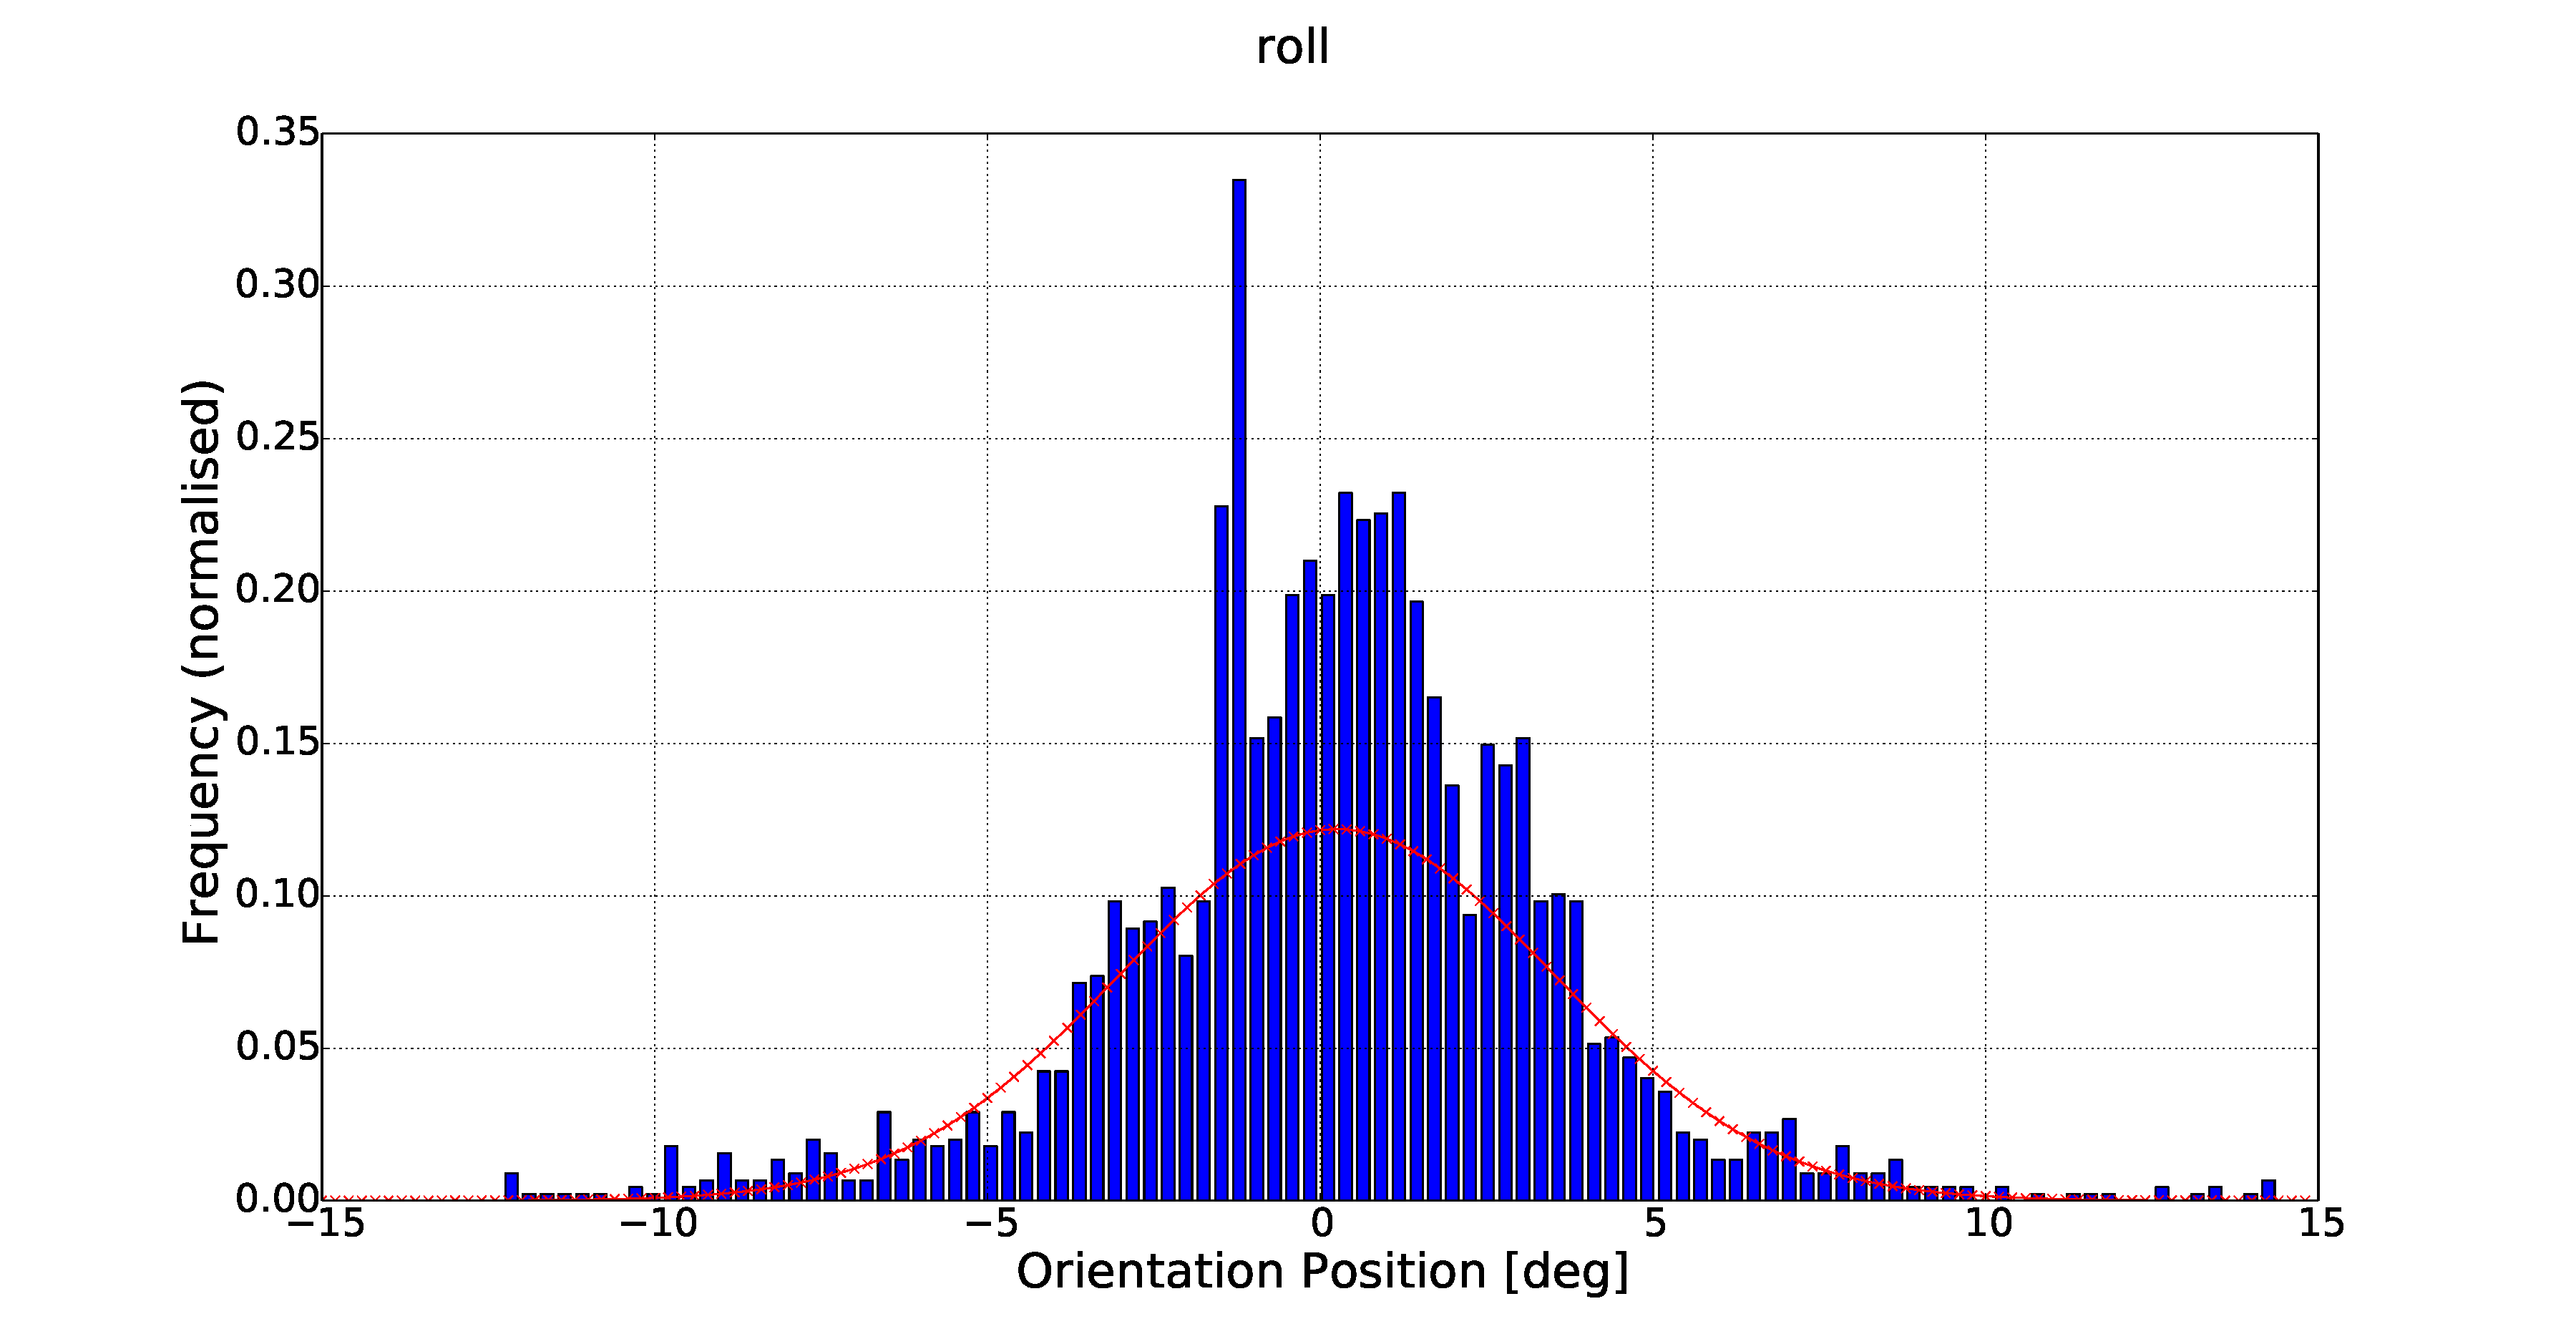
\includegraphics[clip, trim = 150 50 155 0, width=\textwidth]{figures/chapter3/norm_roll.pdf}
     %\caption{Histogram of the error in the $\theta$ dimension with a mean of 4 mili-degrees and a standard deviation of 44.0\degree.}
  %\label{fig:norm-roll}
  %\end{subfigure}
%~
  %\begin{subfigure}{0.45\textwidth}
     %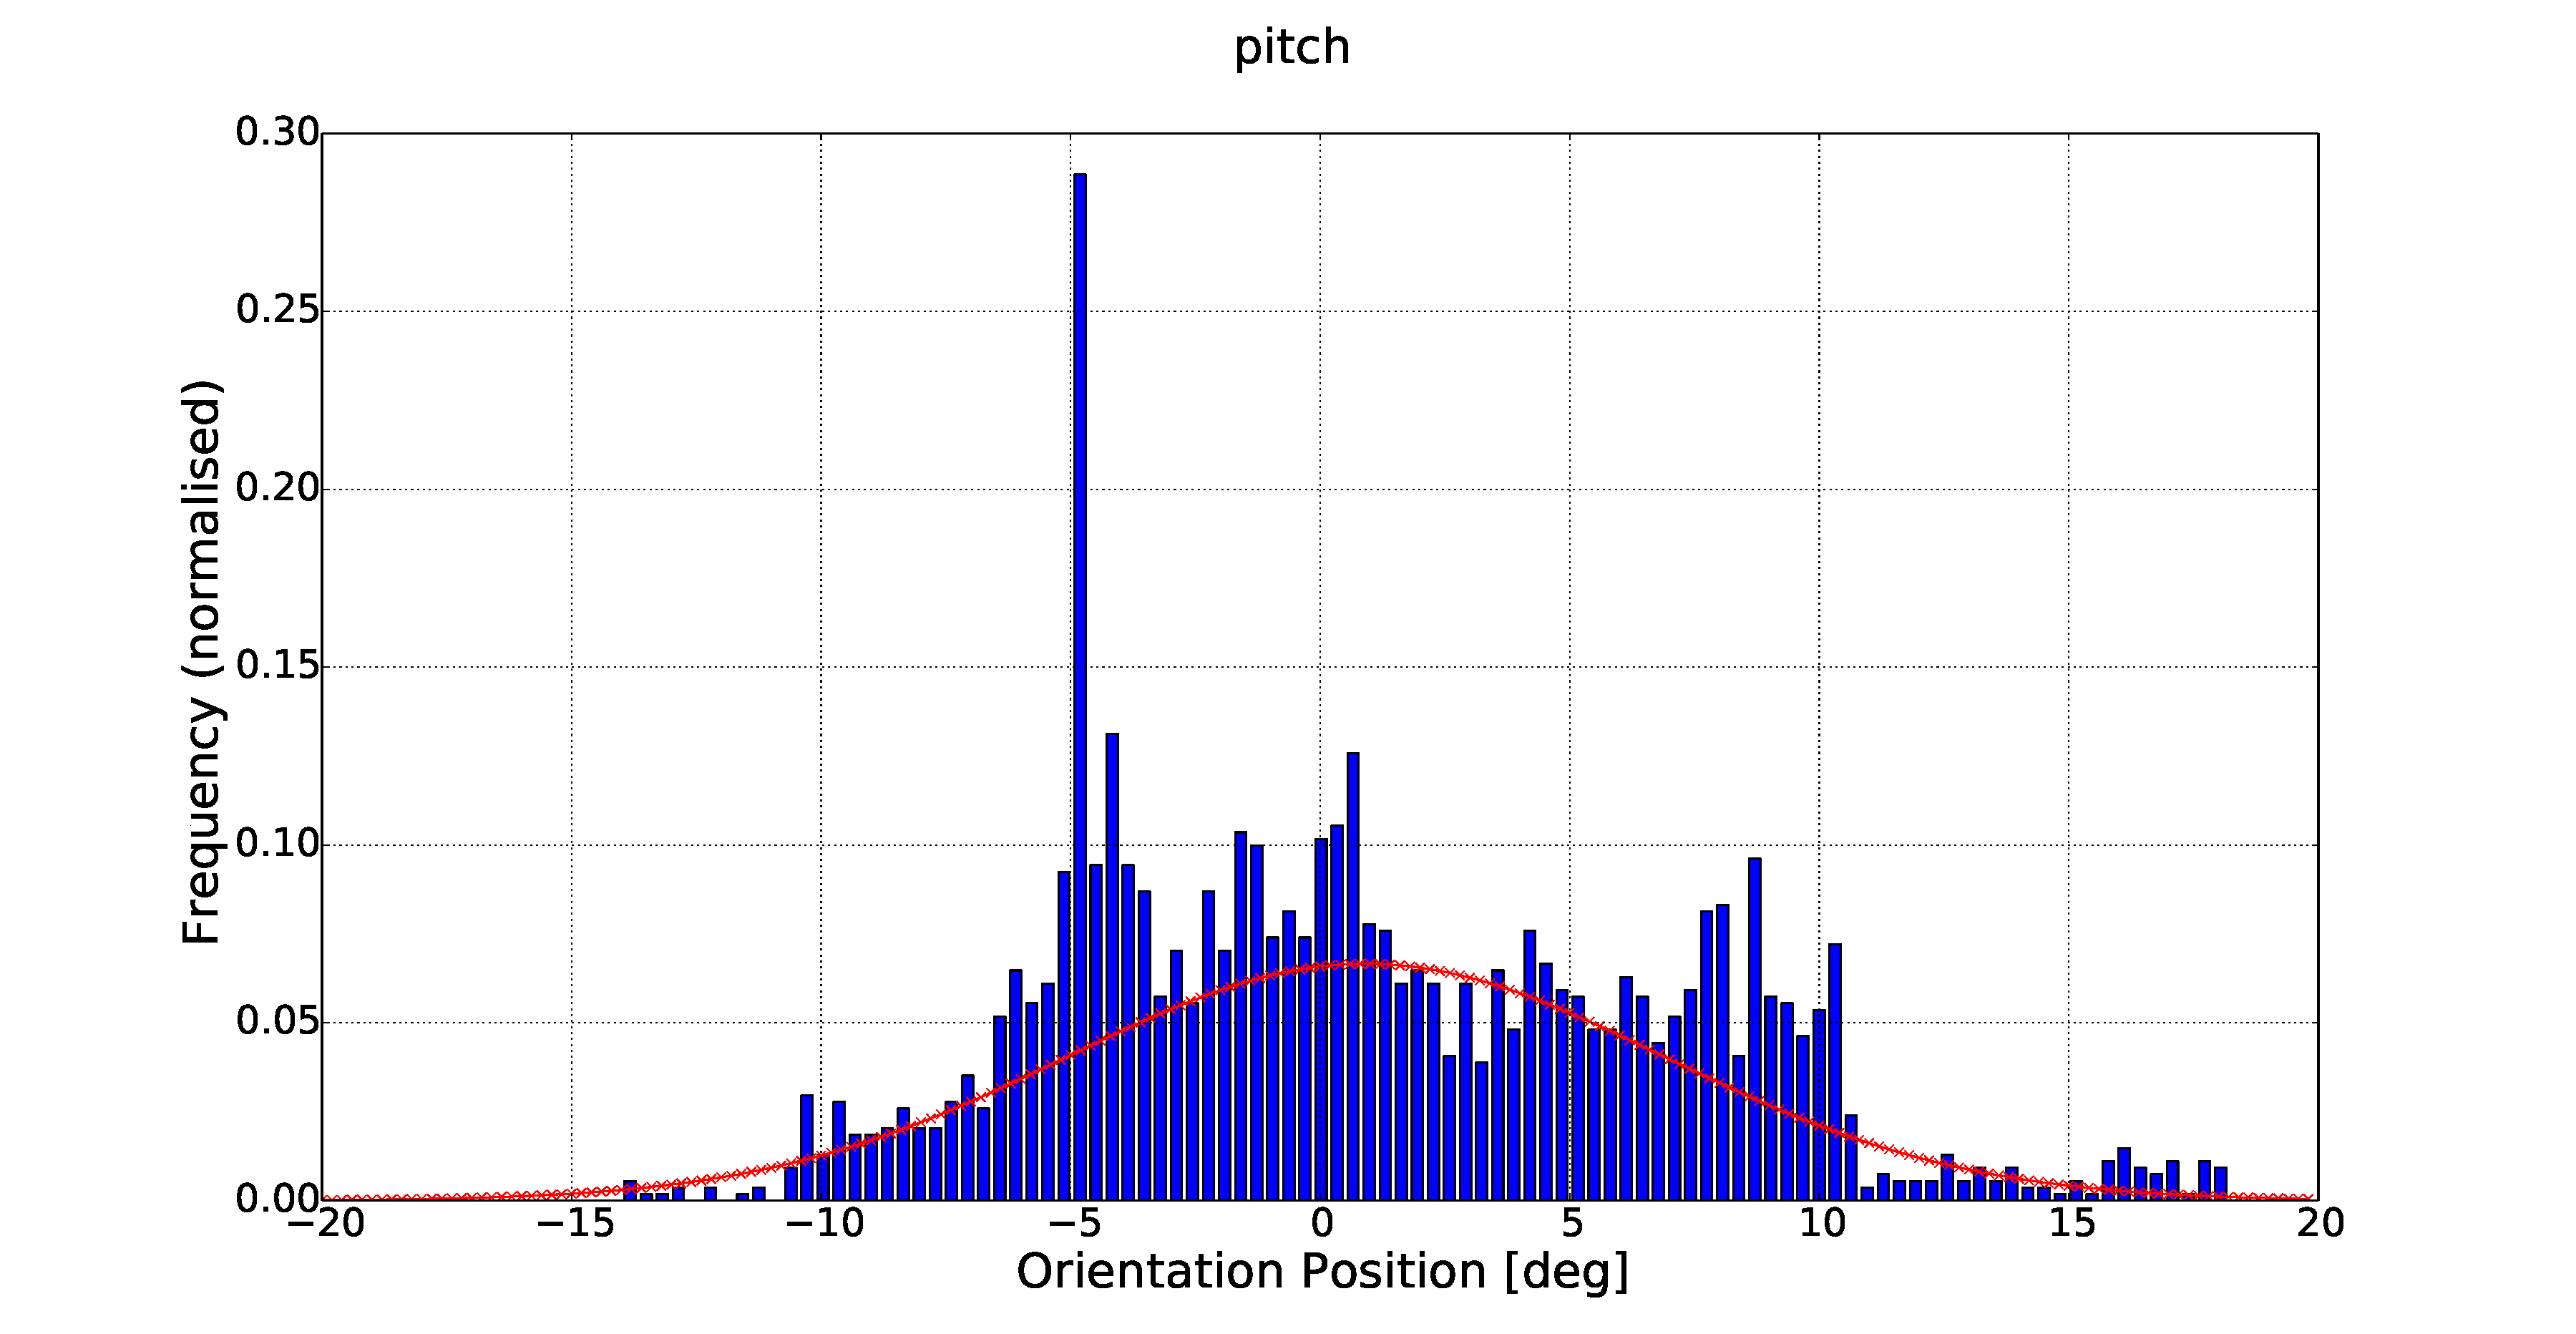
\includegraphics[clip, trim = 150 50 155 0, width=\textwidth]{figures/chapter3/norm_pitch.pdf}
     %\caption{emem}
  %\label{fig:norm-pitch}
  %\end{subfigure}
%~
  %\begin{subfigure}{0.45\textwidth}
     %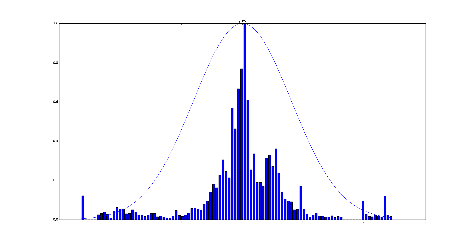
\includegraphics[clip, trim = 150 50 155 0, width=\textwidth]{figures/chapter3/norm_yaw.pdf}
     %\caption{memememe}
  %\label{fig:norm-yaw}
  %\end{subfigure}
  %\caption{meme}
  %\label{fig:err-norm}
%\end{figure*}

It can be seen that all the plots are roughly centred around 0.0 and are very nearly normally distributed, with the $z$ dimension displaying the largest standard deviation of approximately 500mm. Again, a bad depth estimate is to be expected when working with a single camera.

In all, the histograms of the errors show that the assumption made in Equation~\ref{eq:offset} that the errors are normally distributed around 0.0 is a valid one. 

\subsection{Optimum Focal Lengths and Offset}

As a result of the focal length and offset optimisation process, the optimal focal lengths, $f_x$ and $f_y$ were found to be 628 and 535 after 50 iterations, which is considerably less than the optimum of 700 produced by OpenCV's calibration toolbox. Note that these units are given in camera pixel units and not millimetres. The optimal offset $\bar{\bm{P}}$ was found to be approximately

\[
  [240.8mm, \; 40.09mm, \; 375.9mm, \; \ang{184.3}, \; \ang{-2.697}, \; \ang{-179.9}]^T
\]

The values in $\bar{\bm{P}}$ contain any constant error bias that may have been introduced to the system during testing. The offsets in the $\theta$ and $\psi$ dimensions can be explained by the differing axis orientations of the CVS camera and Vicon systems, reorienting it by approximately $\pm$180\degree. This indicates that the offset was correctly calculated and is doing what it is supposed to. The large offset in the $z$ dimension is to be expected, since single camera's are known to produce very bad depth estimates. The offset of 240mm in the $x$ dimension is slightly surprising. However, it may be explained when it is considered that the origin of the chessboard and camera are on opposite sides when facing each other. The chessboard's origin would be four blocks, or 400mm, away from the camera's along the $x$-axis, making up for the 320mm offset.

All of the above produce an error 2-norm of approximately 0.81 (normalised), compared to the original 1.15, normalised. Figures~\ref{fig:estimate-x} to~\ref{fig:estimate-yaw} show the results of the Vicon measurements compared to the original and improved CV system measurements in all 6 dimensions.

%\begin{figure*}
  %\begin{subfigure}{0.45\textwidth}
    %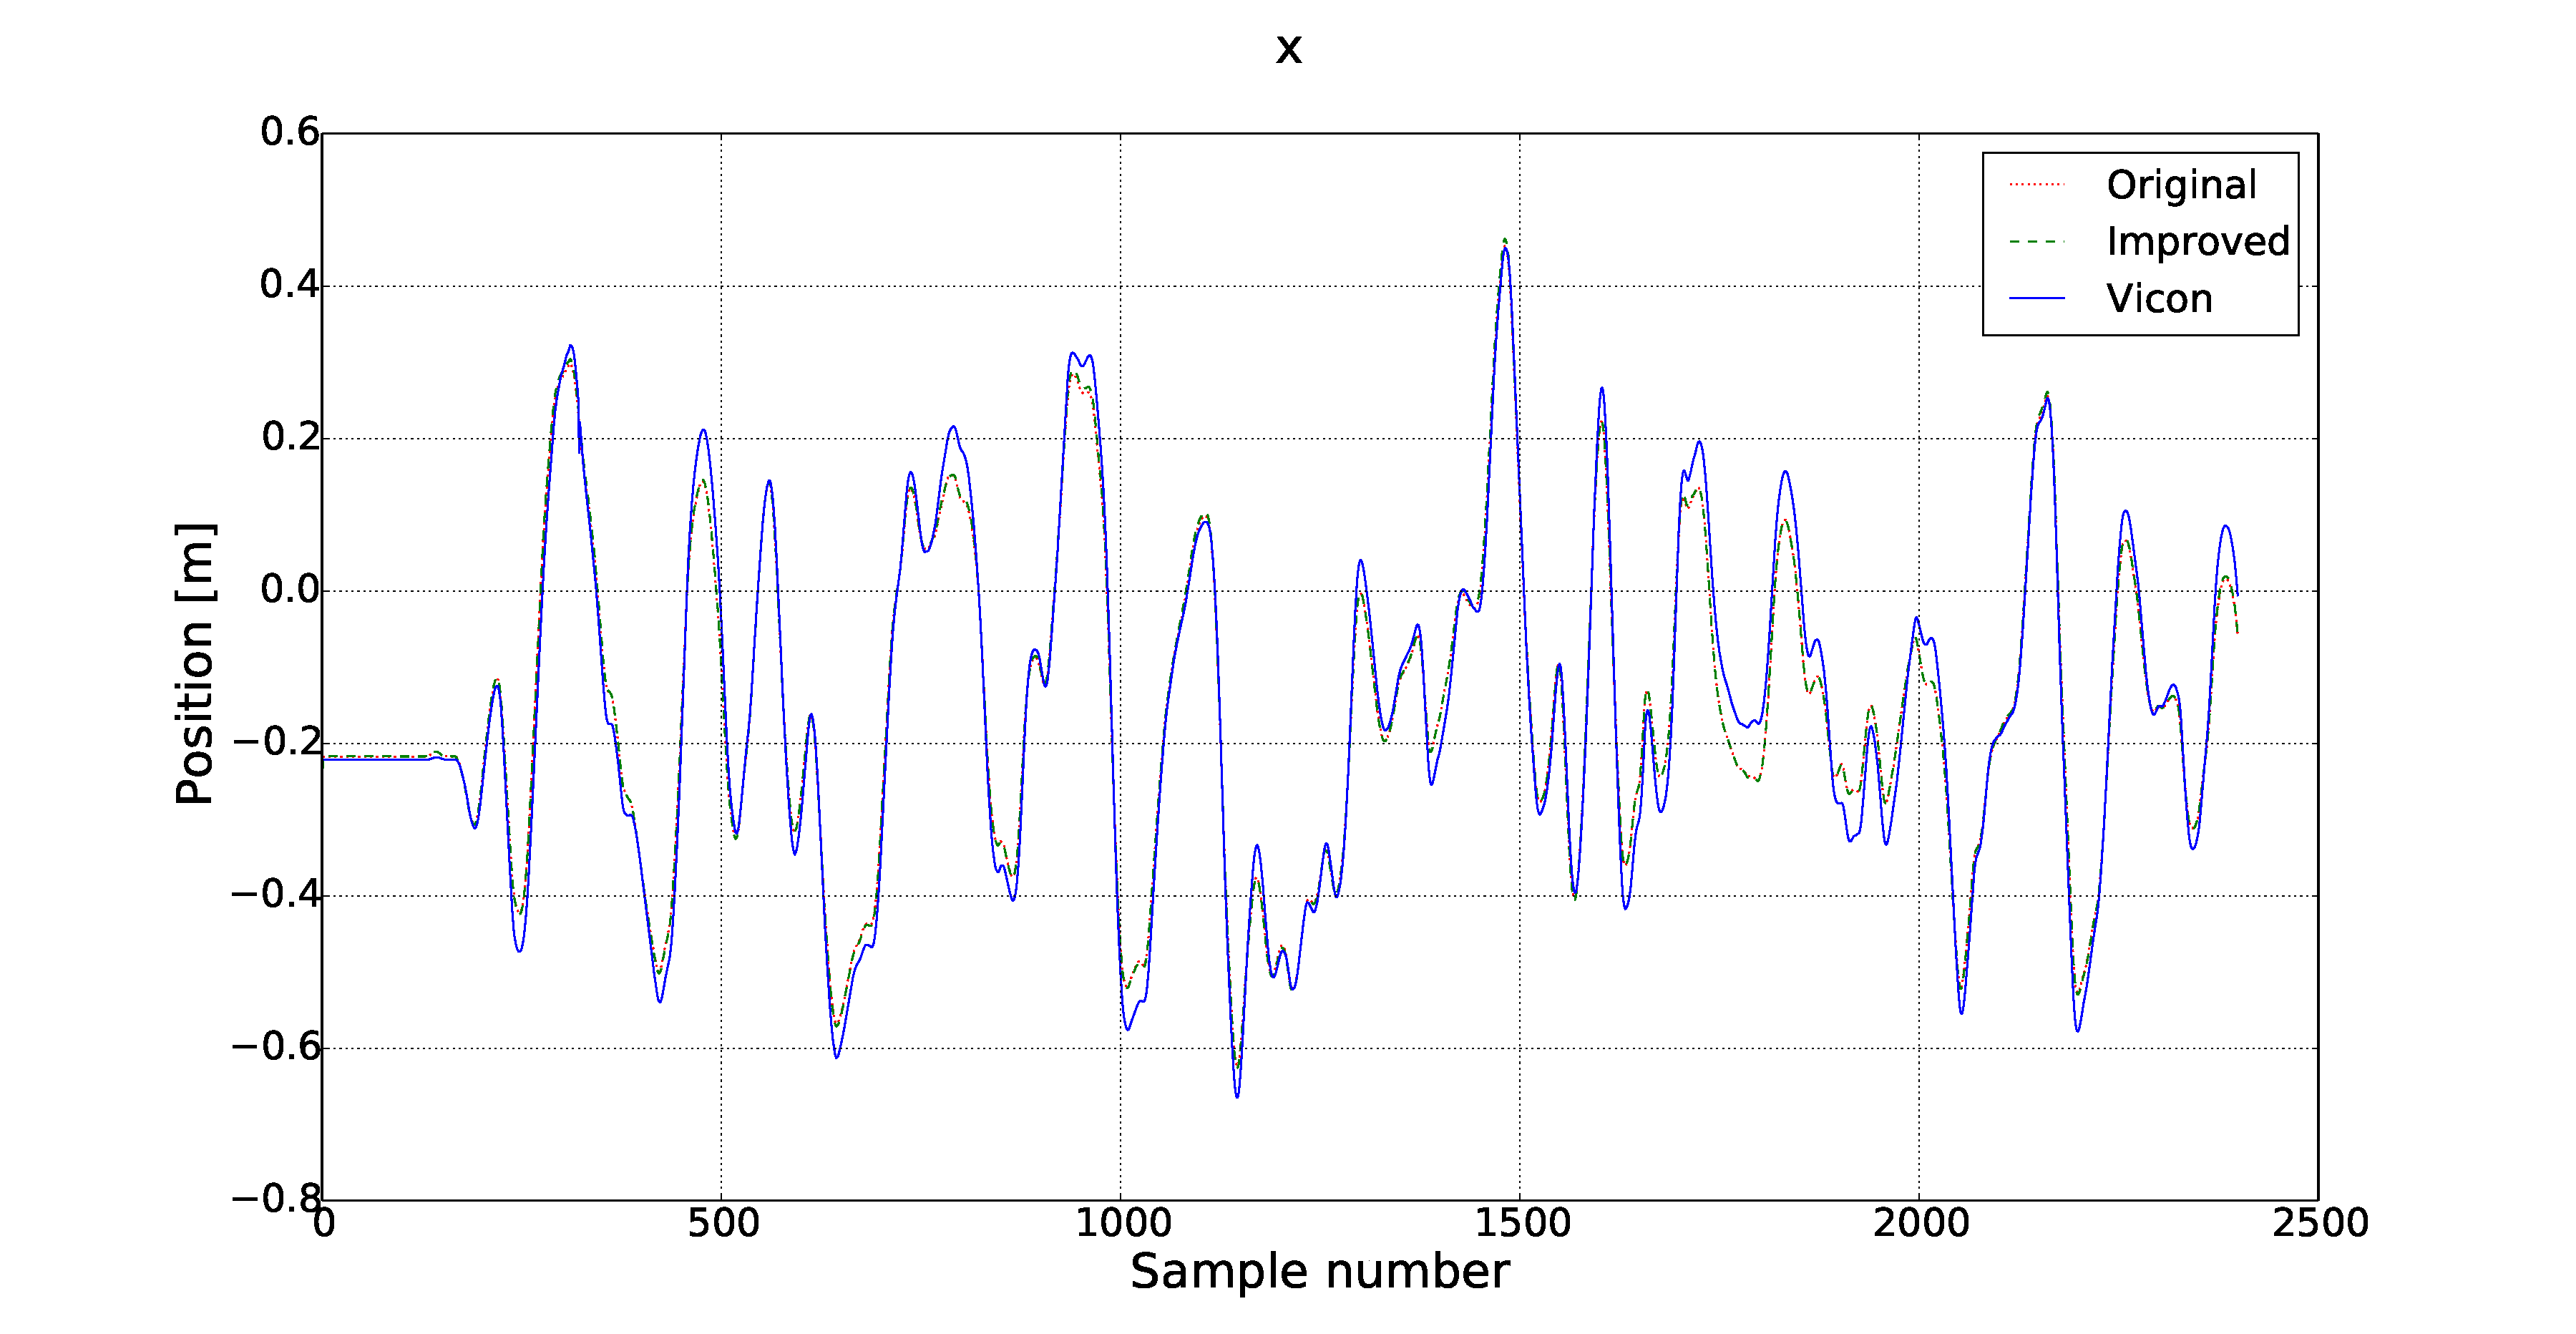
\includegraphics[clip, trim = 200 50 150 0, width=\textwidth]{figures/chapter3/x}
    %\caption{The ground-truth Vicon pose estimate, versus the original and improved CV pose estimates in the $x$ dimension.}
  %\label{fig:estimate-x}
  %\end{subfigure}
%~
  %\begin{subfigure}{0.45\textwidth}
    %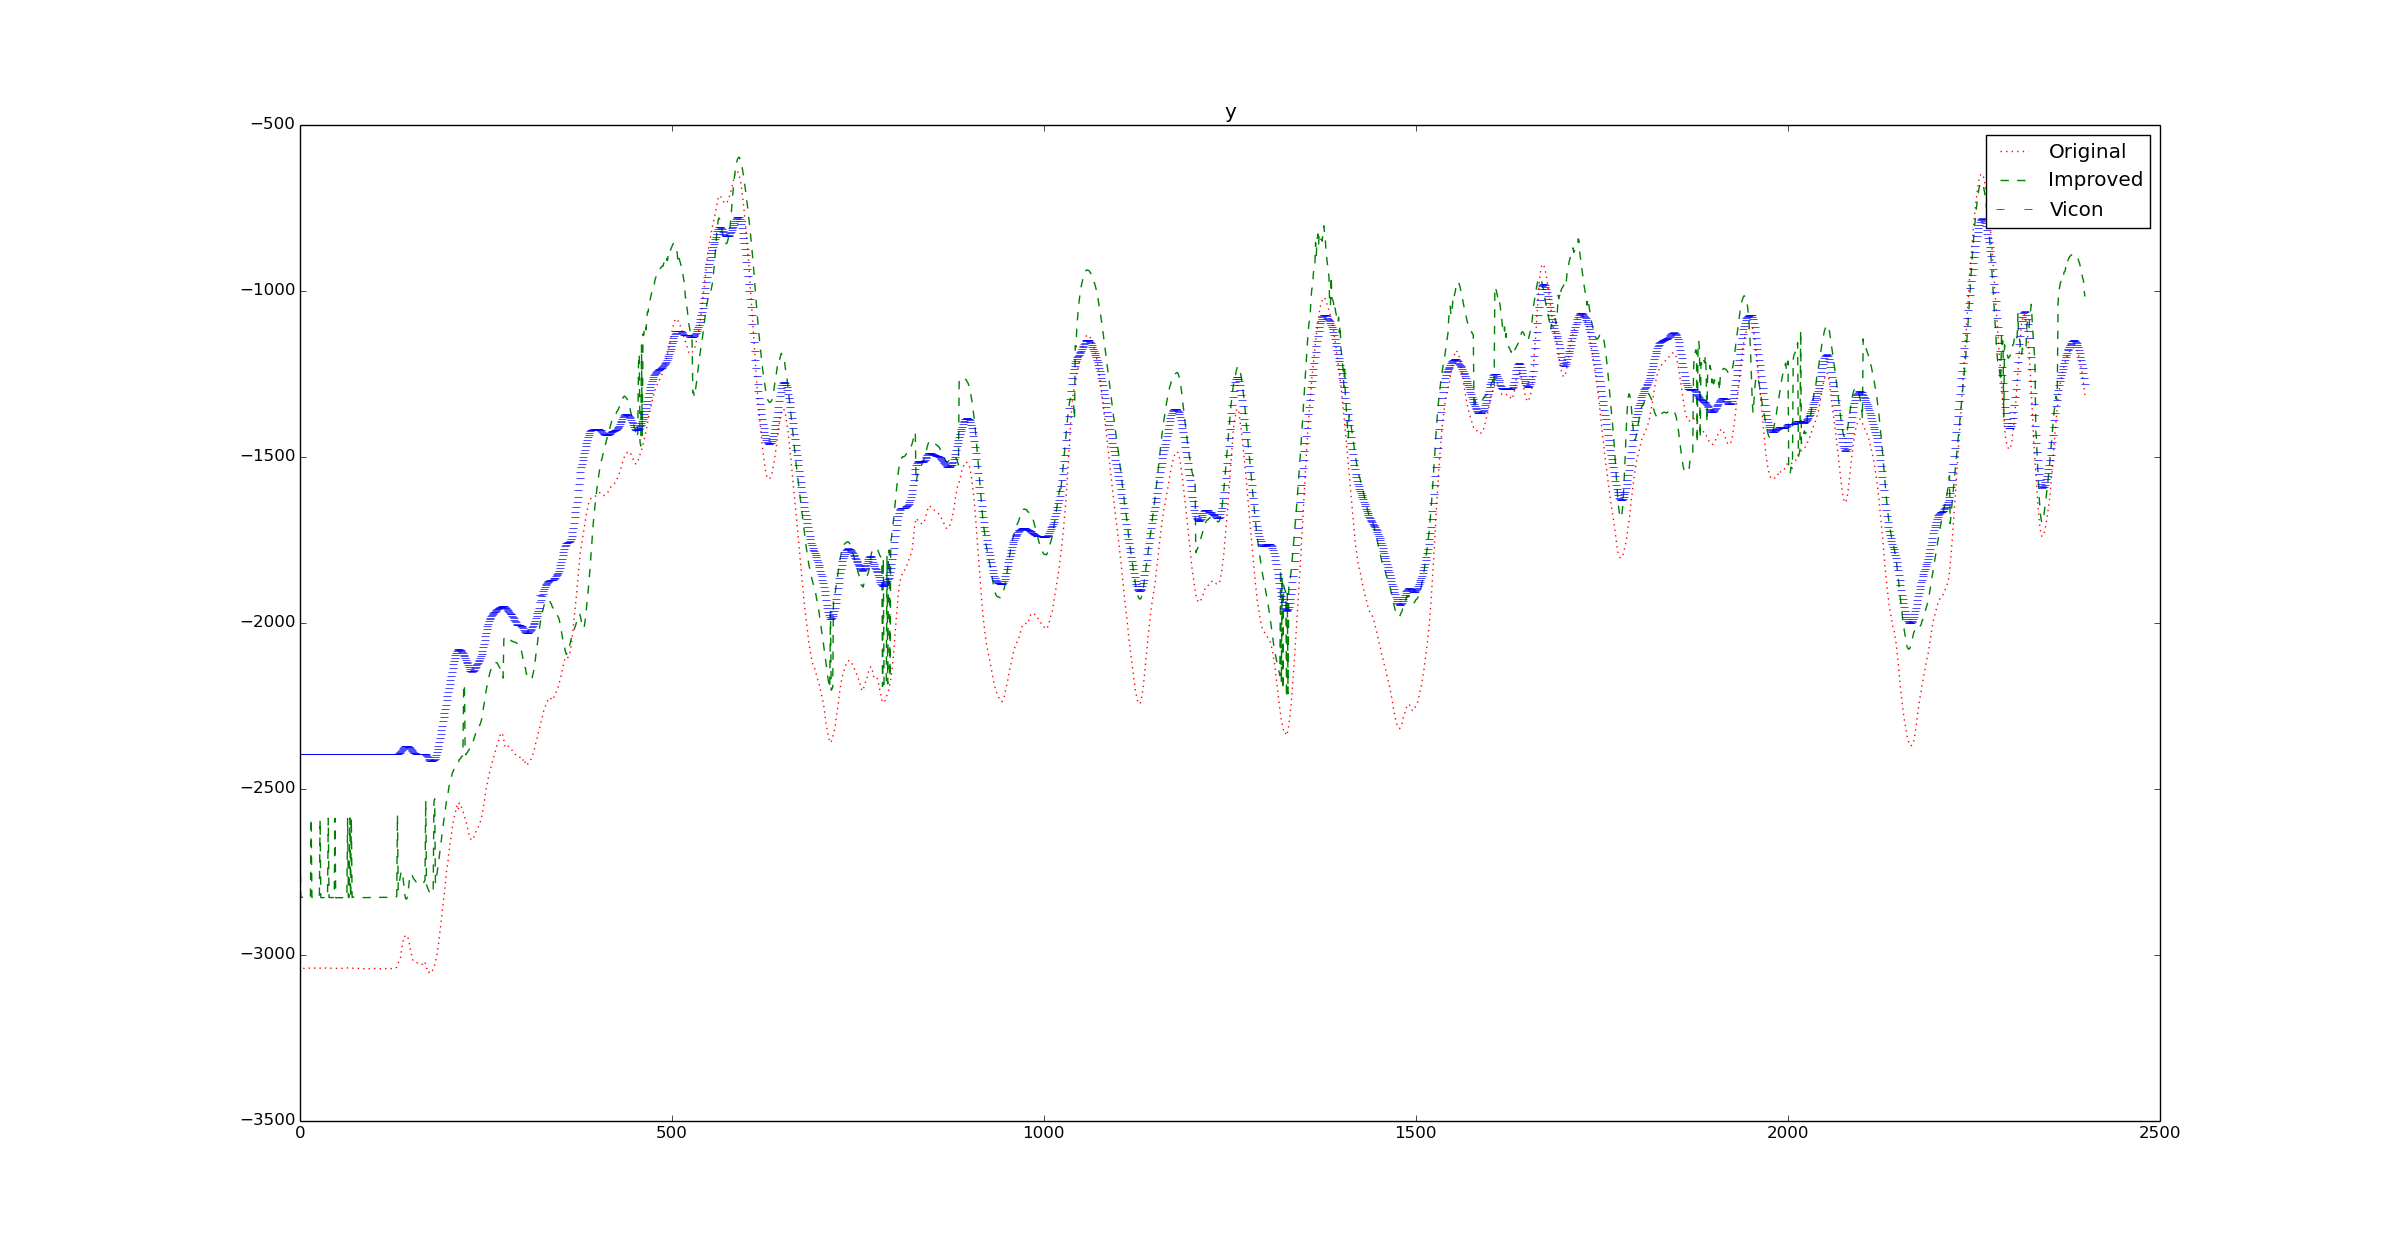
\includegraphics[width=\textwidth]{figures/chapter3/y}
    %\caption{The ground-truth Vicon pose estimate, versus the original and improved CV pose estimates in the $y$ dimension.}
  %\label{fig:estimate-y}
  %\end{subfigure}
%~
  %\begin{subfigure}{0.45\textwidth}
    %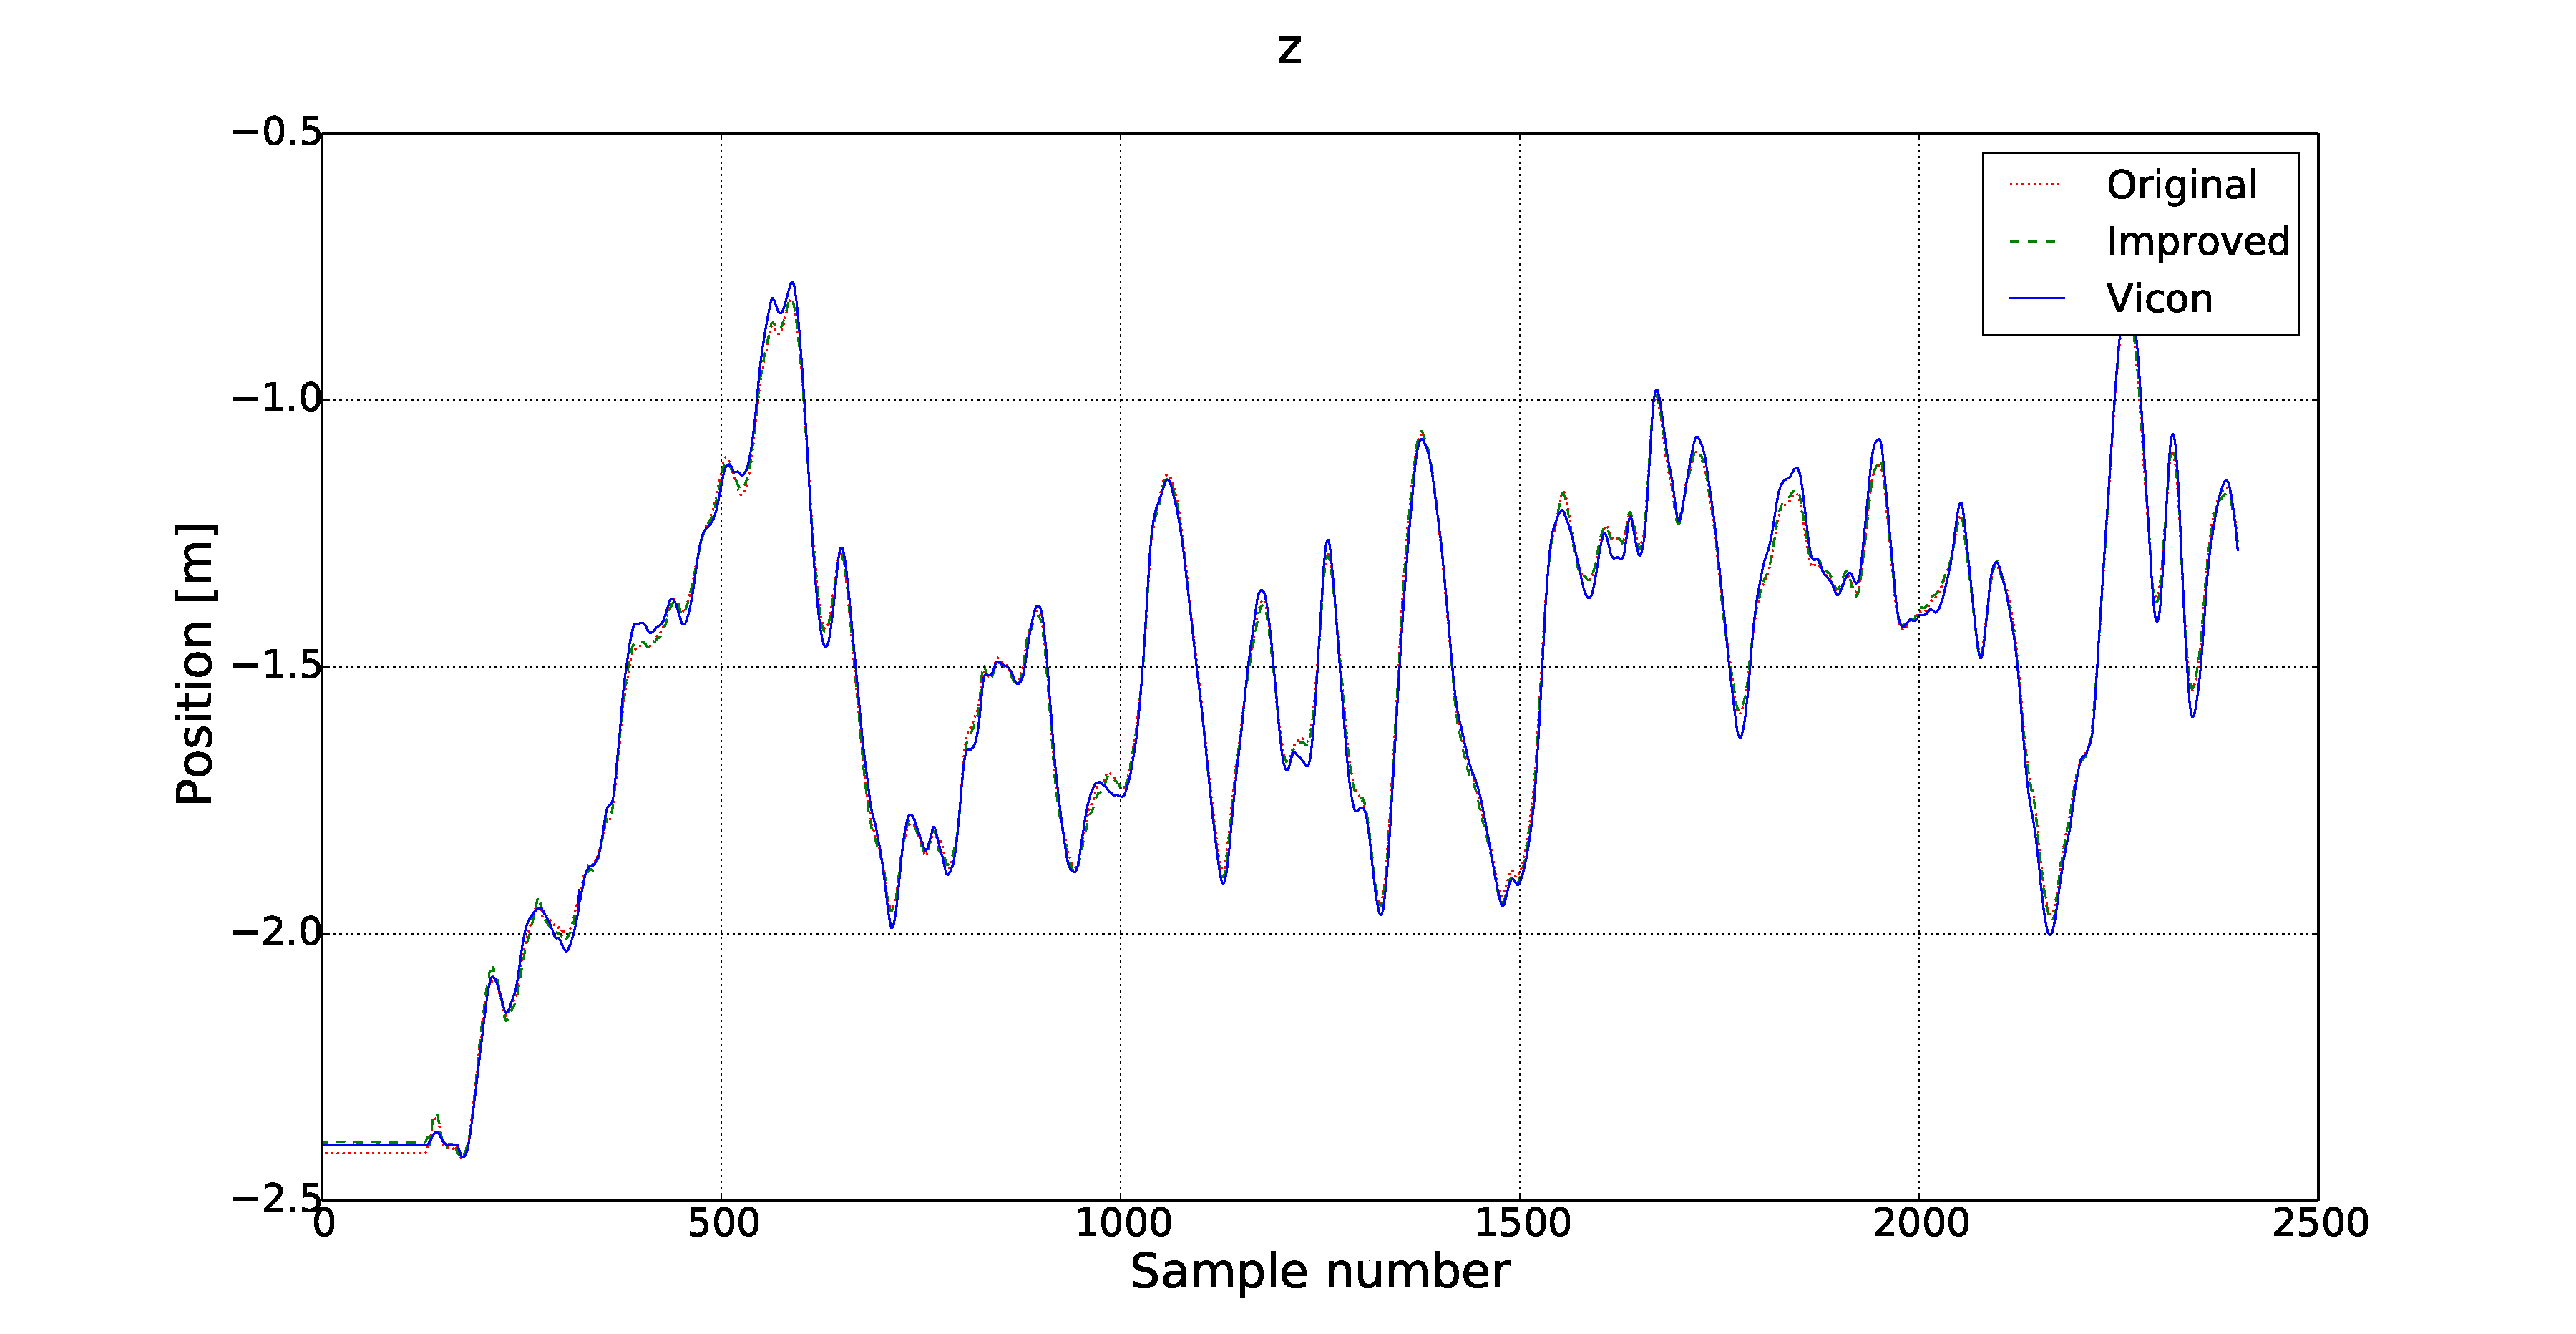
\includegraphics[width=\textwidth]{figures/chapter3/z}
    %\caption{The ground-truth Vicon pose estimate, versus the original and improved CV pose estimates in the $z$ dimension.}
  %\label{fig:estimate-z}
  %\end{subfigure}
%~
  %\begin{subfigure}{0.45\textwidth}
    %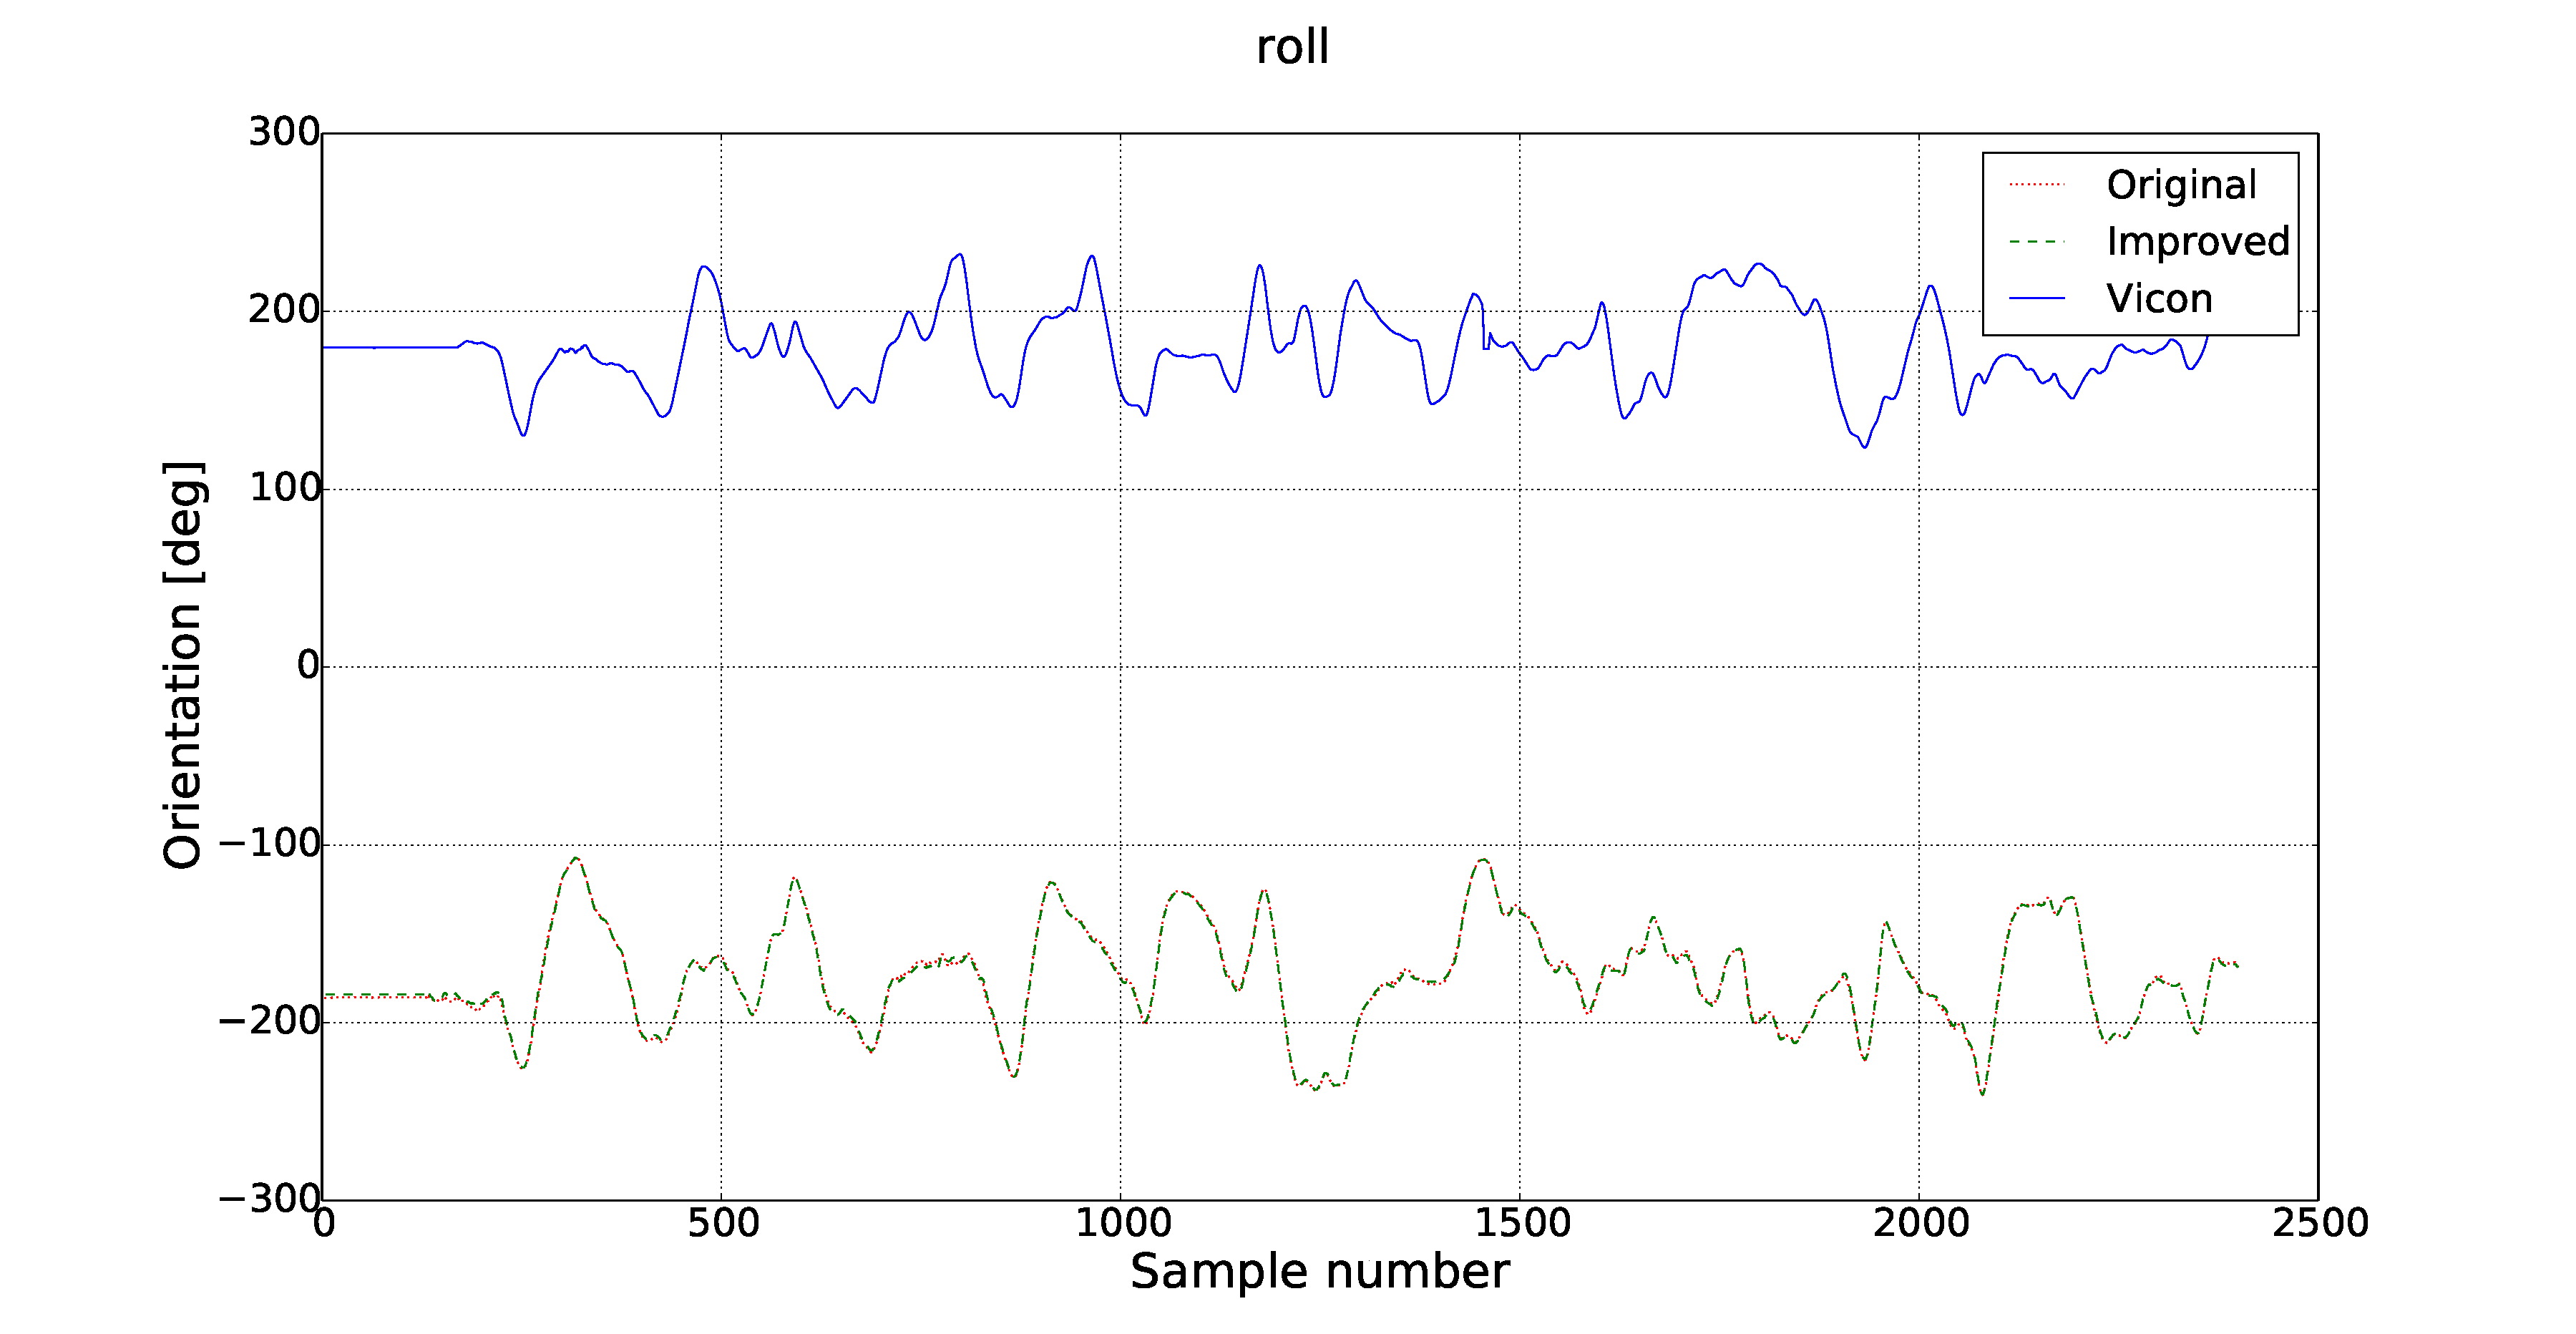
\includegraphics[width=\textwidth]{figures/chapter3/roll}
    %\caption{The ground-truth Vicon pose estimate, versus the original and improved CV pose estimates in the $\theta$ dimension.}
  %\label{fig:estimate-roll}
  %\end{subfigure}
%~
  %\begin{subfigure}{0.45\textwidth}
    %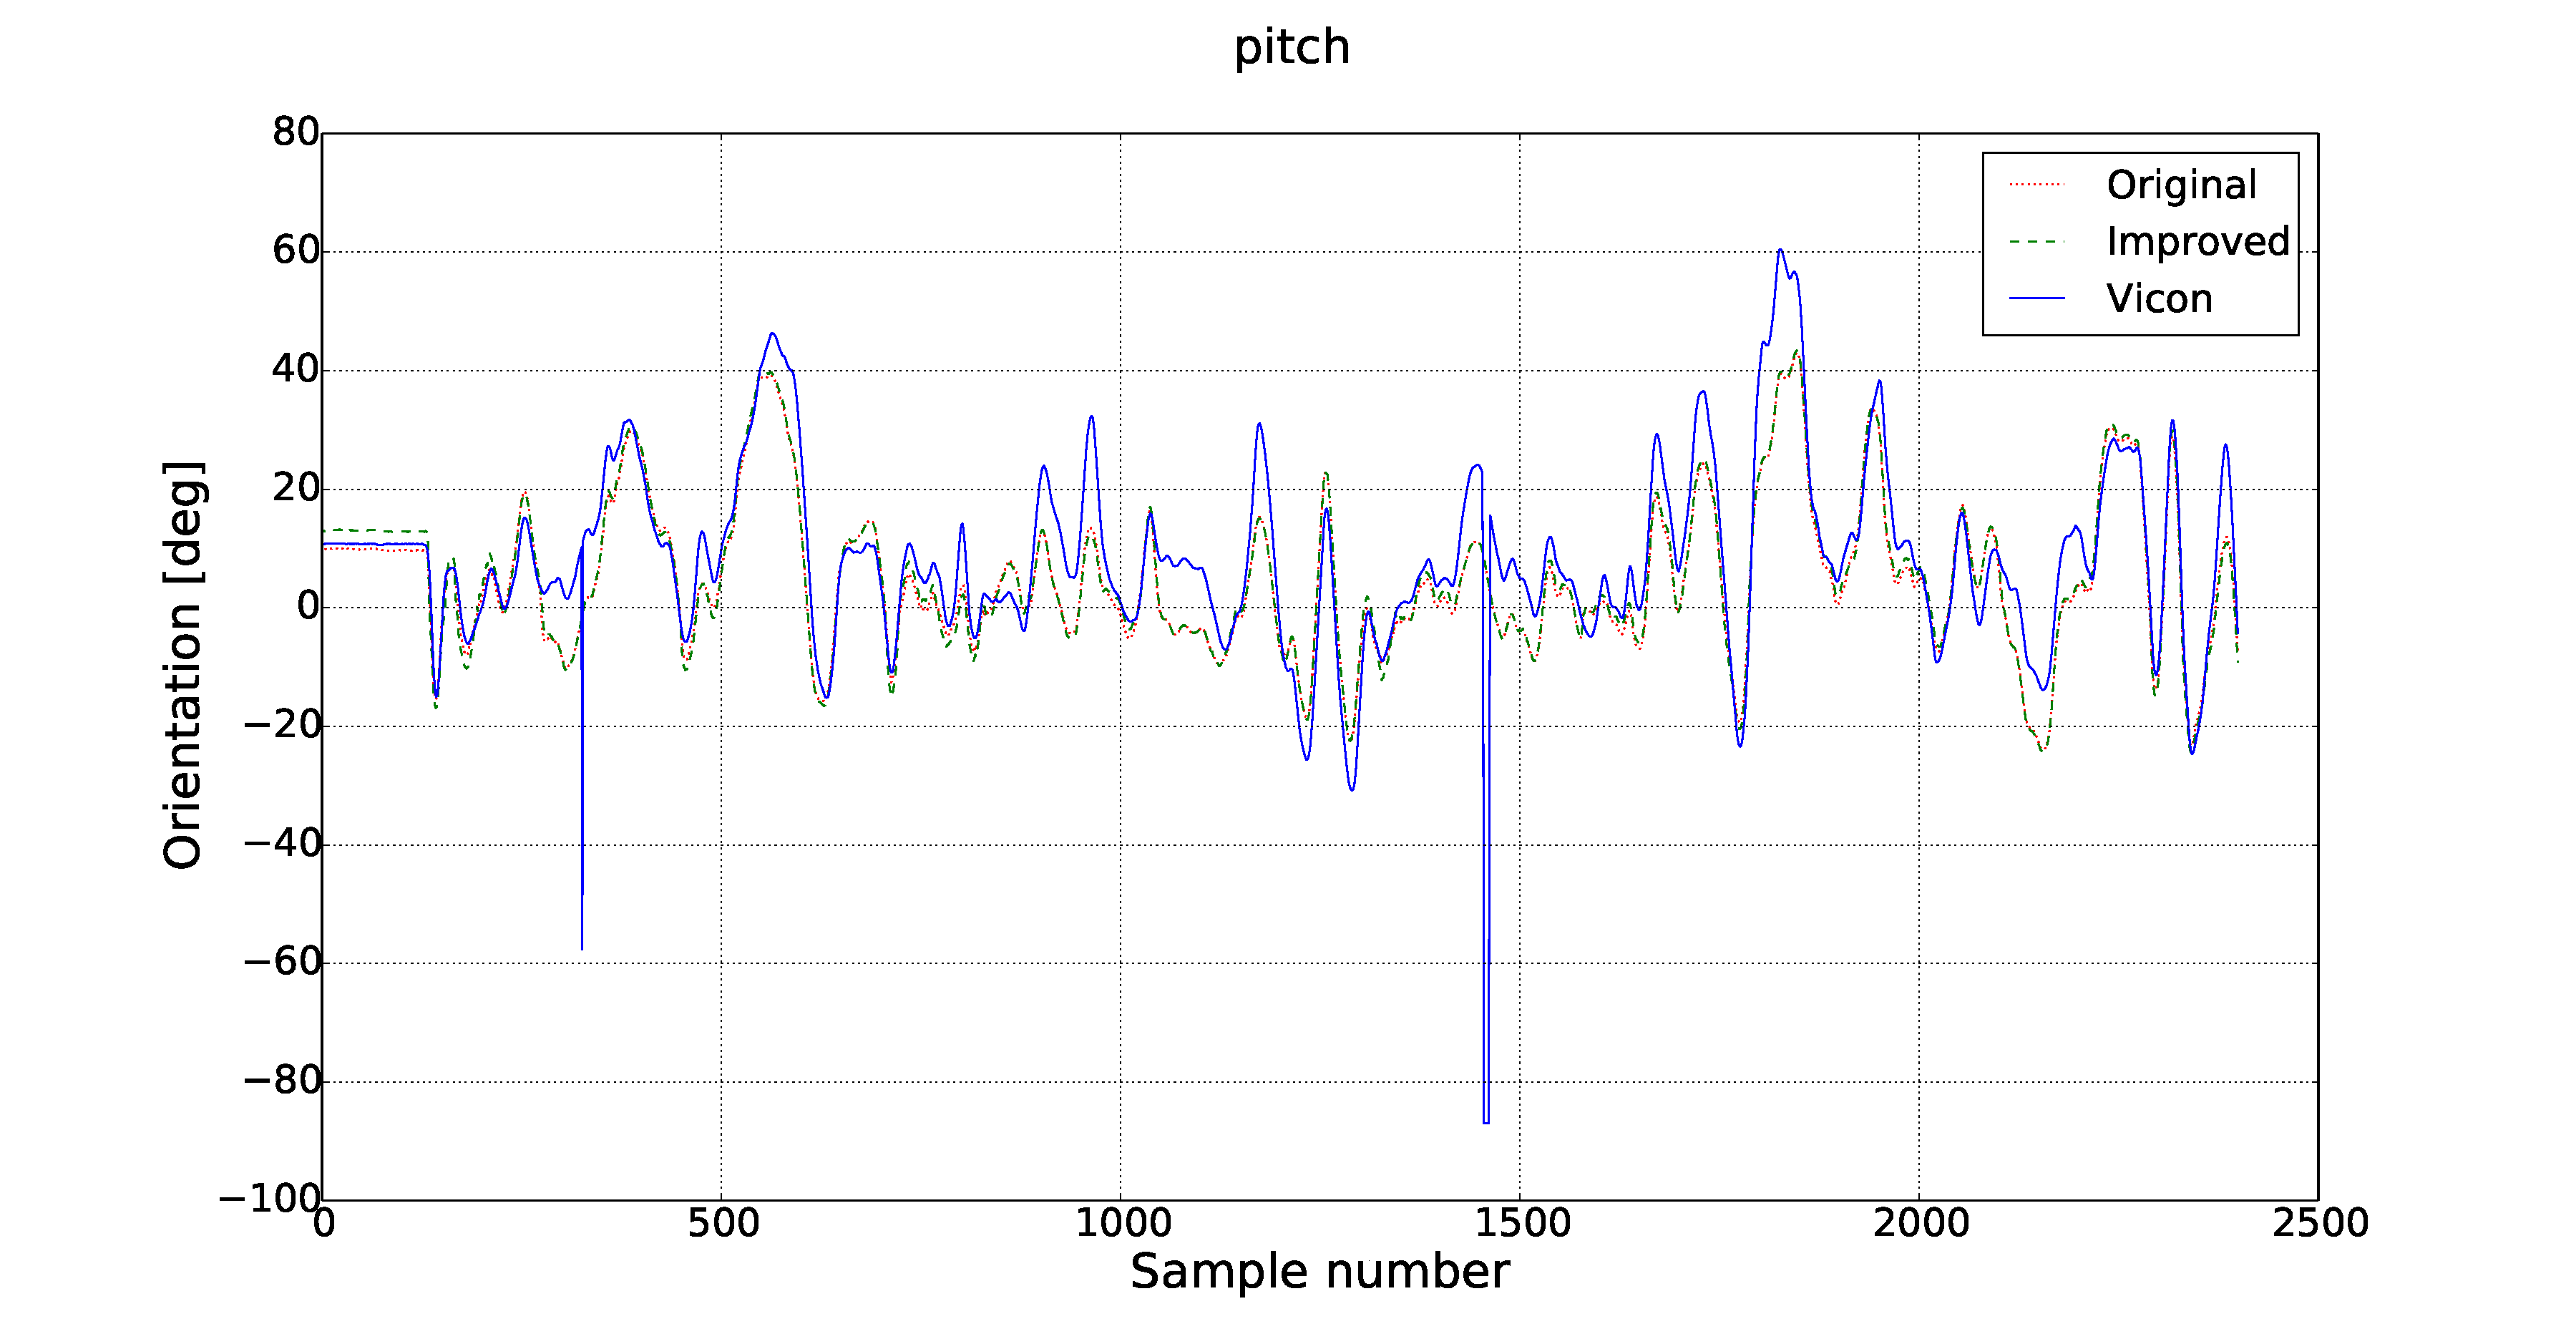
\includegraphics[width=\textwidth]{figures/chapter3/pitch}
    %\caption{The ground-truth Vicon pose estimate, versus the original and improved CV pose estimates in the $\phi$ dimension.}
  %\label{fig:estimate-pitch}
  %\end{subfigure}
%~
  %\begin{subfigure}{0.45\textwidth}
    %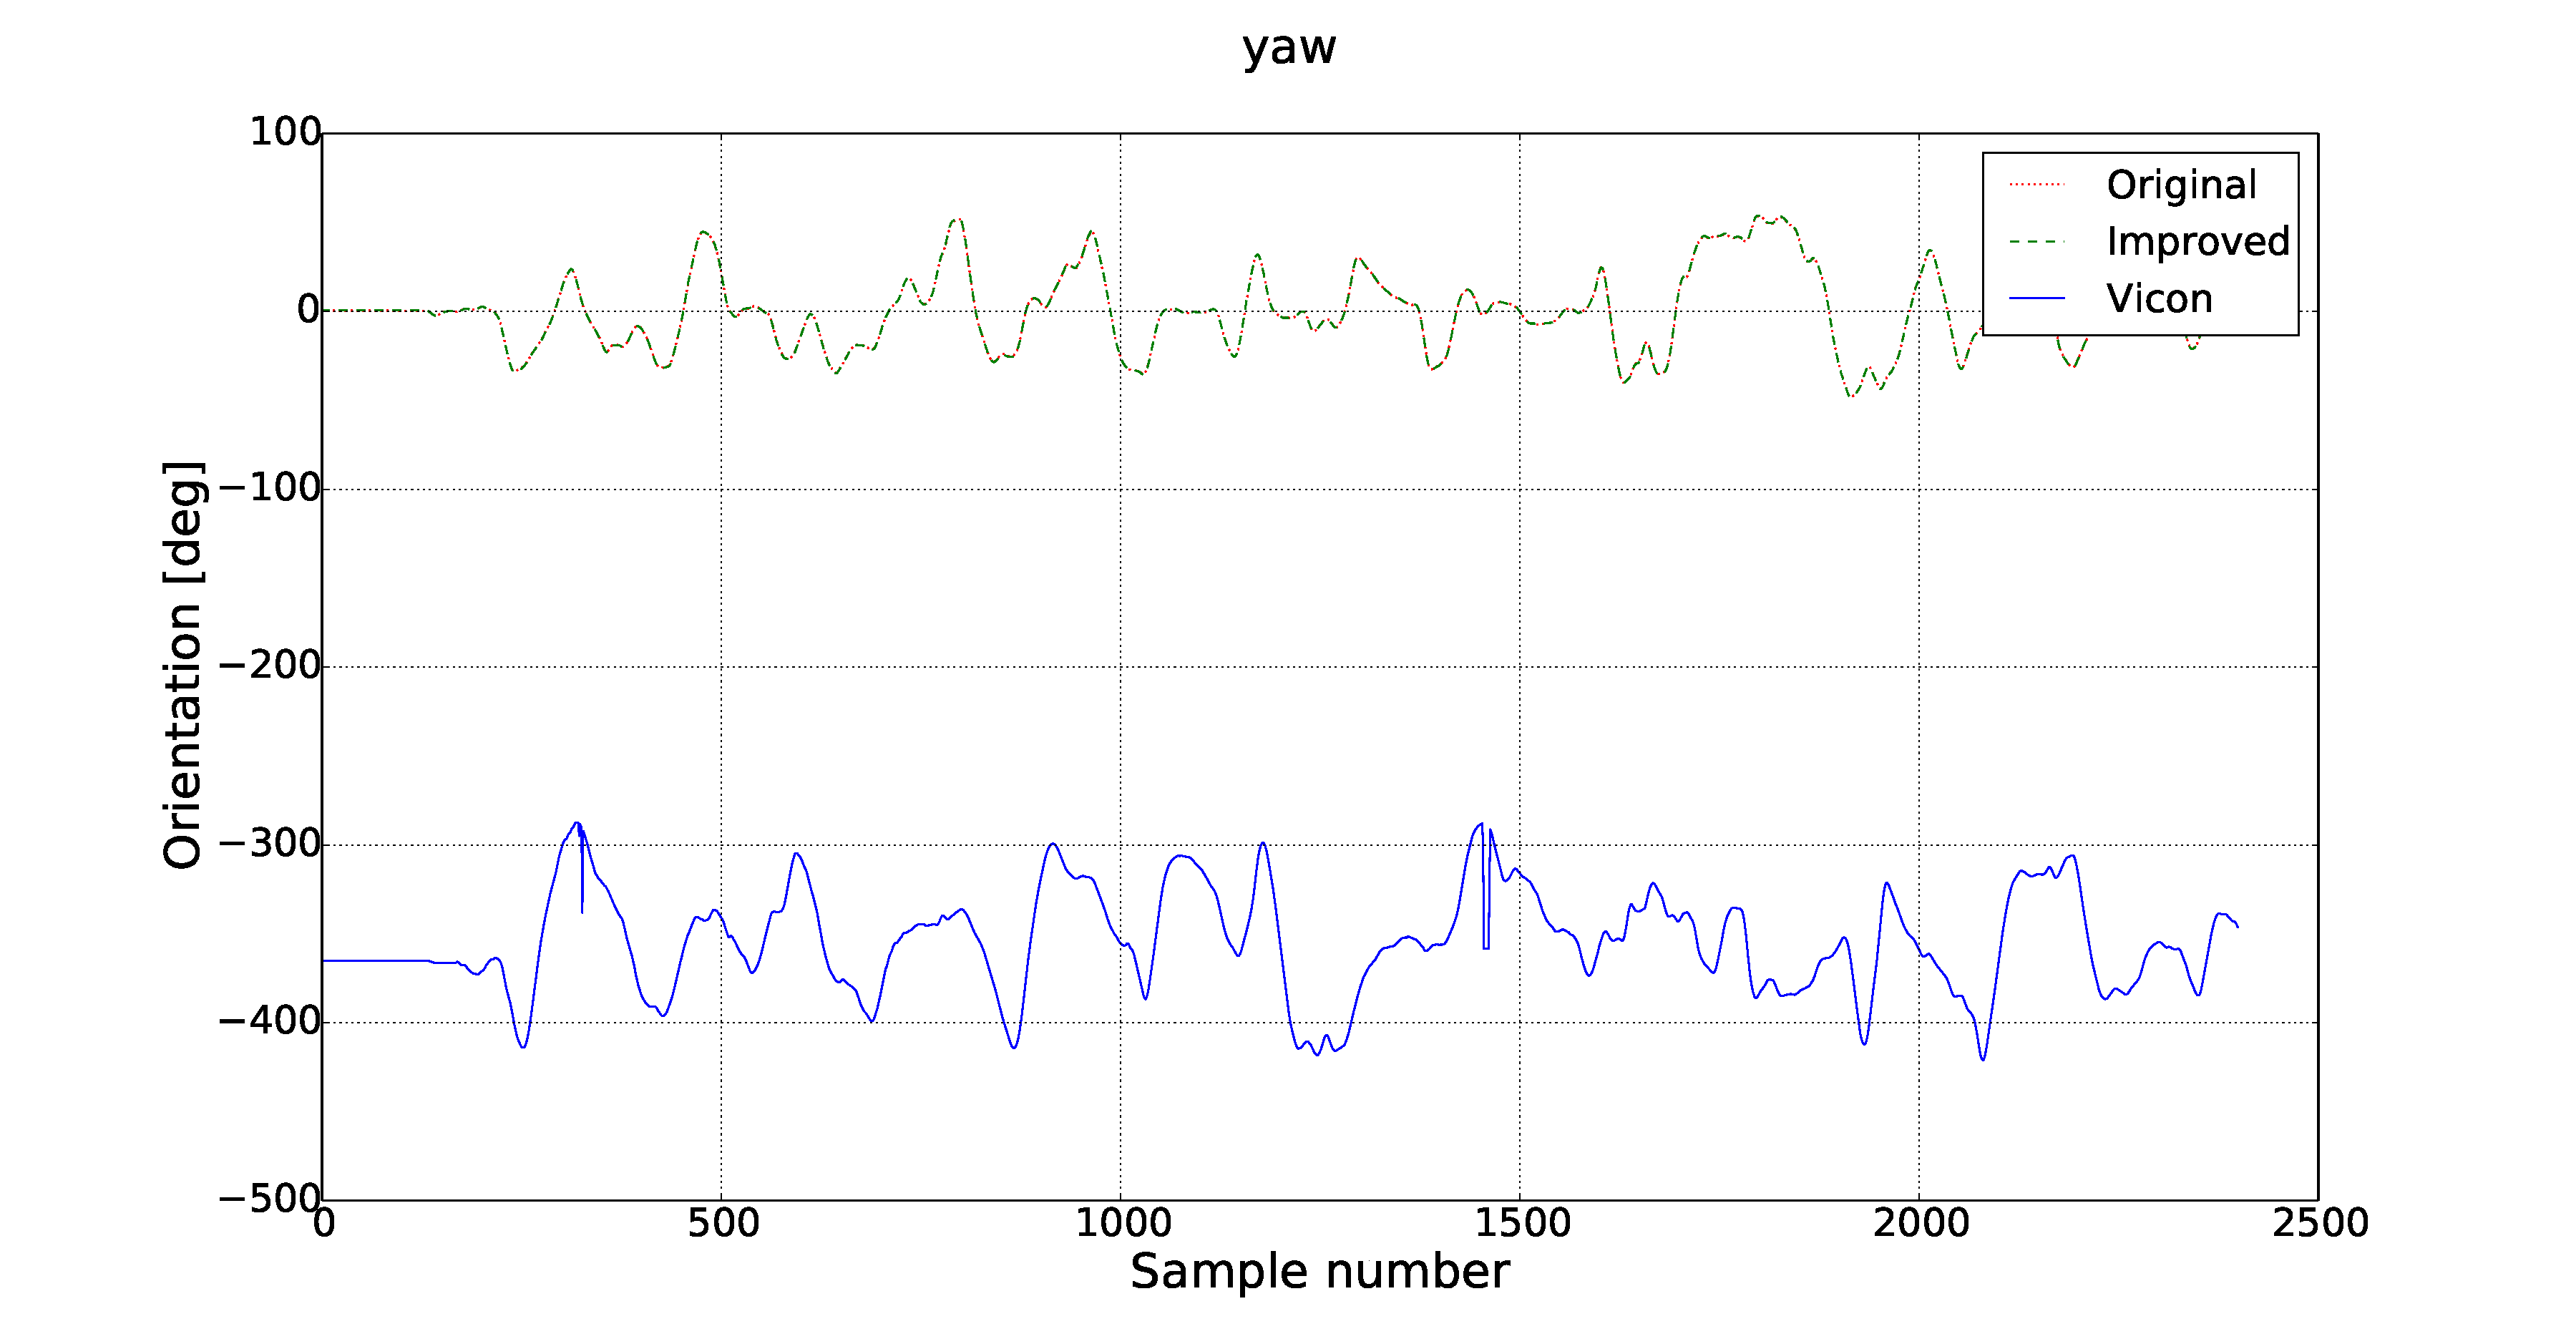
\includegraphics[width=\textwidth]{figures/chapter3/yaw}
    %\caption{The ground-truth Vicon pose estimate, versus the original and improved CV pose estimates in the $\psi$ dimension.}
  %\label{fig:estimate-yaw}
  %\end{subfigure}
%\end{figure*}

It can be seen that there is a some improvement in all the dimensions. However, in some cases the improvement is negated by worse results in another place in the data set. This is a result of the optimisation process where an improvement at timeframe $t_i$ in the $x$ dimension, for example, may lead to a worse estimate at time $t_i$ in the $\phi$ dimension. Since the norm of $\bm{\epsilon}$ converges, it can be taken that the improved results are indeed better as a whole, even though it may look like it has gotten worse in the individual dimensions.

\subsection{System Accuracy}

Determining the accuracy of a multi-dimensional model is often a complex task, but the fact that the error is normally distributed makes it possible to use the covariance matrix to check the interdimensional variance and dependence. If it is found that the diagonal of the covariance matrix is sufficiently large relative to the off-diagonal elements, the dimensions can be taken as strongly enough independent of one another and the variance along the diagonal can be taken as a measure of the accuracy. 

The covariance matrix, $\bm{\Sigma}$, was found to be 

\[
  \bm{\Sigma} = 
  \begin{bmatrix}
    \bm{3131.7} & 2255.2 & 98.227 & 94.371 &  98.830 & 106.85 \\ 
    2255.2 & \bm{40924}  & 4038.2 & 197.46 &  30.631 & 1953.7 \\
    98.227 & 4038.2 & \bm{5592.5} & 241.75 &  106.86 & 385.23 \\
    94.371 & 197.46 & 241.75 & \bm{84.939} &  10.303 & 13.792 \\
    98.830 & 30.631 & 106.86 & 10.303 &  \bm{110.54} & 63.381 \\
    106.85 & 1953.7 & 385.23 & 13.792 &  63.381 & \bm{318.17} \\
  \end{bmatrix}
\]

The matrix $\bm{\Sigma}$ shows that there are large off-diagonal elements, indicating that there is strong interdimensional dependence. This unfortunately means that there is no clear indication on the accuracy of the system. However, a probability density function (PDF) can be set up using $\bm{\Sigma}$ that will show what the expected error in the 6 dimensions will be for a given pose. The PDF is given by Equation~\ref{eq:pdf}.

\begin{equation}
  \label{eq:pdf}
  p(\bm{\epsilon}) = \frac{1}{\sqrt{{(2\pi)}^k\lvert\bm{\Sigma}\rvert}}e^{-\frac{1}{2}{(\bm{\epsilon} - \bm{\mu})}^T\bm{\Sigma}^{-1}(\bm{\epsilon} - \bm{\mu})}
\end{equation}

Armed with a PDF and covariance matrix, it is now possible to determine whether the CV system is more accurate than the on-board sensor suite of a drone. 

\section{Conclusion}

